% ======================================================================
%  AI for Economics and the Economics of AI
%  Zhigang Feng (University of Nebraska--Omaha)
%
%  Version 13: reference list halved (224 -> 113 entries); seven
%  regulatory documents now cited in footnotes. October 2026.
%  Section 5.2 and
%  Appendix B rest on the March 2026 release of the Anthropic Economic
%  Index and lead with the direction of the deployment skew.
%  Compile:  xelatex survey_restructured_v13.tex ;
%            biber survey_restructured_v13 ; xelatex (x2)
%  Bibliography: references.bib + references_supplement.bib
% ======================================================================
\documentclass[12pt]{article}

% -------------------- engine & fonts --------------------
\usepackage{iftex}
\ifPDFTeX
  \usepackage[T1]{fontenc}
  \usepackage[utf8]{inputenc}
  \usepackage{lmodern}
\else
  \usepackage{fontspec} % XeLaTeX/LuaLaTeX: Latin Modern by default
  % Drafting CJK fallback: renders Chinese glyphs in a few bib entries and
  % in-text place names. Harmless if the fonts are absent.
  \IfFileExists{xeCJK.sty}{%
    \usepackage{xeCJK}%
    \IfFontExistsTF{FandolSong-Regular.otf}{\setCJKmainfont{FandolSong-Regular.otf}}{%
      \IfFontExistsTF{Noto Serif CJK SC}{\setCJKmainfont{Noto Serif CJK SC}}{%
        \IfFontExistsTF{PingFang SC}{\setCJKmainfont{PingFang SC}}{}}}%
  }{}
\fi

% -------------------- language & quotes --------------------
\usepackage[american]{babel}
\usepackage{csquotes}

% -------------------- page & spacing --------------------
\usepackage[margin=1in]{geometry}
\usepackage{setspace}
\onehalfspacing

% -------------------- math --------------------
\usepackage{amsmath, amssymb, amsthm, mathtools, bm}

% -------------------- graphics & tables --------------------
\usepackage{graphicx}
\graphicspath{{figures/}}
\usepackage{booktabs, array}
\usepackage{xcolor}
\usepackage{tikz}
\usetikzlibrary{arrows.meta, positioning, calc, shapes.geometric}

\usepackage{microtype}
% Second-pass stretch so long unbreakable tokens (URLs, model names)
% do not produce overfull lines.
\emergencystretch=1.5em

% -------------------- bibliography --------------------
\usepackage[backend=biber, style=authoryear-comp, natbib=true,
            maxcitenames=3, maxbibnames=10, giveninits=false,
            uniquename=false, uniquelist=false,
            isbn=false, doi=true, url=true, sortcites=true]{biblatex}
\addbibresource{references.bib}
\addbibresource{references_supplement.bib}
% AEA-style citations: no comma between author and year.
\renewcommand*{\nameyeardelim}{\addspace}
\setcounter{biburlnumpenalty}{9000}
\setcounter{biburllcpenalty}{9000}
\setcounter{biburlucpenalty}{9000}

% Colored, clickable citations (blue); internal links plain; URLs blue.
\usepackage[colorlinks=true, citecolor=blue, linkcolor=black,
            urlcolor=blue]{hyperref}

% -------------------- theorem / box environments --------------------
\theoremstyle{plain}
\newtheorem{proposition}{Proposition}[section]
\theoremstyle{definition}
\newtheorem{definition}[proposition]{Definition}
\newtheorem{assumption}[proposition]{Assumption}
\theoremstyle{remark}
\newtheorem{remark}[proposition]{Remark}

% -------------------- metadata --------------------
\title{AI for Economics and the Economics of AI\thanks{%
Feng: Department of Economics, University of Nebraska--Omaha
(\href{mailto:zfeng@unomaha.edu}{zfeng@unomaha.edu}).
I am most grateful to Yili Chien, Bo Li, Xiaojie Liu, Udara Peiris, Yaolang Zhong, Luofeng Zhou, Mohan Zhou, and Shenghao Zhu for comments and discussions. I thank Max Quint for editorial help. This paper supersedes and replaces the author's earlier working paper
``Artificial Intelligence in Economics: Tools, Transformations, and
Methodological Innovations'' \citep{Feng2025AIEcon}.
The author acknowledges support from UCRCA at the University of
Nebraska--Omaha and NNSF of China (Grant Nos.~72450003 and 72433004). This work was completed using the facilities at the
NCSA at the University of Illinois, supported by the NSF's ACCESS program under grant no. SOC250017.
}}
\author{Zhigang Feng}
\date{October 2026}

\begin{document}

\maketitle

\begin{abstract}
\noindent
Artificial intelligence is changing both how economists conduct
research and the economic processes they study: it is a toolkit for
measurement, prediction, identification, and computation, and an
economic force acting on production, work, and growth. This survey
connects the two roles through intelligence as a produced factor:
cognitive services produced by models trained on data and compute,
traded separately from human labor, and partly fed by their own output.
We review the research toolkit and the evidence on labor markets,
market power, and governance, and develop four open questions: how the
factor is produced and what a model learns from records, where it is
deployed within occupations, how its output is verified and directed,
and how its use feeds back to future capability. The last is the
Middle-Intelligence Trap, a stagnation risk in which degraded training
data and weakened human expertise reinforce one another while
corrective investment lags. New descriptive evidence from 253 U.S.
occupations links AI usage concentrated on core tasks to lower
employment growth in the Current Population Survey; the association is
conditional, depends on sample coverage, and does not appear in payroll
data. A stylized model identifies a verification externality when
corrections reach later training and benefit users beyond those who pay
for them.

\medskip

\noindent\textbf{JEL codes:} C45, C55, D24, D82, J24, O33, O40.\\
\textbf{Keywords:} artificial intelligence; machine learning; large language
models; factor of production; data economics; verification.
\end{abstract}

\newpage

% =====================================================================
% Section 1 -- Introduction
% =====================================================================
\section{Introduction}

Artificial intelligence is changing both how economists conduct
research and the economic processes they study. As an
instrument, it changes how economists gather data, form predictions,
identify causal effects, solve models, and read text at scale. As an
object, it is reshaping labor markets, the distribution of income and
power, and the institutions through which economies are governed. The
scale of the second change shows in investment plans and in use: projected
U.S. investment in data
centers and the chips and power behind them runs to several percent of
GDP a year over 2025--2032, on average a larger share of output than the
railroad build-out absorbed \citep{VanNieuwerburgh2026BrookingsAICapex},
and generative AI has been adopted faster than the personal
computer or the internet were at comparable stages of their diffusion
\citep{BickBlandinDeming2025}. Nor
are the two changes separate subjects: the technology with which an
economist nowcasts output from satellite images and news articles is the
technology whose labor-market consequences the economist is trying to
measure. This survey treats them as one subject and asks what is new
about each.

Our organizing answer is that AI makes intelligence increasingly
available as a \emph{produced} factor. Models trained on data with large amounts of compute increasingly supply cognitive services apart from any particular worker's
time; language-model services are often billed by the token. Model
parameters and reusable outputs are non-rival information goods;
producing new inference consumes rival compute and energy. The factor
also participates in its own reproduction: generated output can enter
later training, so current selection and verification decisions can
affect future capability. Deployed as agents, however, these systems also raise problems of
direction and coordination. Cognition has long entered economic theory
as a constraint, human capital, and an input to research. The change is
the breadth of learned services that can be reproduced outside the
person. As generation becomes cheaper, scarcity moves both toward the inputs
that produce the factor (compute, energy, informative data) and toward
the complements its use requires (verification and judgment). Following
those moving scarcities is the thread that runs through the survey.

Read as a toolkit (Section~\ref{sec:ai-for-econ}),
AI has earned its
place in applied economics where flexible, data-driven approximation
was the binding constraint: measurement and nowcasting from
high-dimensional and unstructured data, causal inference with
machine-learning first stages, and the solution and estimation of rich
heterogeneous-agent models. With text now treated as data, large language
models extend the toolkit further, to annotation, research assistance,
and simulated experimental subjects. Across these
applications, cheaper computation relocates the economist's judgment
rather than retiring it: the scarce inputs become the framing of
questions, the identification strategy, the economic structure imposed,
and the validation of what a model has and has not learned.

Read as an object (Section~\ref{sec:econ-of-ai}), this survey analyzes AI
as a general-purpose technology: it is pervasive, technologically
dynamic, and creates complementarities with downstream innovation, the
criteria of \citet{BresnahanTrajtenberg1995}, which
\citet{BrynjolfssonRockSyverson2019} argue AI meets. Its incidence is uneven
and in places novel. Measured exposure rises with skill and pay rather than staying
confined to routine work. Scale economies in data and compute favor
concentration, though they do not guarantee that any one provider keeps
its lead. Opaque decision systems raise
problems of bias, accountability, and surveillance that the price
mechanism does not resolve on its own. Throughout, we read the evidence
against the three governance approaches reviewed below,
drawing in particular on the Chinese record of platform, algorithm, and
generative-AI rules, which took effect before the European Union's AI
Act obligations began to apply.

The survey's center of gravity is Section~\ref{sec:open}, which
develops four open questions. The first concerns production: what
distinguishes the factor from human and physical capital, what a model
can learn from recorded information, and how to measure useful output
beyond the token. The second presents a \emph{deployment-skew} index
that locates observed AI usage within occupational task bundles. In the
retained household-survey sample, greater concentration on core tasks
is conditionally correlated with lower employment growth. The third
examines verification and direction as generation becomes cheaper.
Instructions cannot state everything a user intends, and behavior also
depends on training, system instructions, and tools. The fourth closes
the loop: unchecked output may degrade later training data, while
delegation may reduce the practice through which evaluative judgment is
formed. Their possible interaction is the Middle-Intelligence Trap.
Appendix~\ref{app:model} formalizes adoption and a verification
externality; it does not establish that the broader trap occurs.

The survey distinguishes synthesis, contributions, and hypotheses.
Sections~\ref{sec:ai-overview}--\ref{sec:econ-of-ai} synthesize
technical, methodological, and economic research. The survey contributes
the produced-factor reading and its connections to recordability,
changing capability, and verification costs; the deployment-skew measure
and descriptive evidence; and the formal framework in
Appendix~\ref{app:model}. Whether limits to learning from records matter
economically, what drives the composition of deployment, and whether the
Middle-Intelligence Trap occurs remain open questions. The last depends on whether independent evaluation stays essential and on how deployment
changes the supply of expertise and informative training data.

Specialized surveys and treatments cover several components:
machine learning for empirical economics \citep{MullainathanSpiess2017,
AtheyImbens2019}, text as data \citep{GentzkowKellyTaddy2019}, deep
learning \citep{Dell2025}, large language models as research tools
\citep{Korinek2023}, the economics of
prediction \citep{AgrawalGansGoldfarb2022}, and AI and growth
\citep{AghionJonesJones2019, Acemoglu2024SimpleMacroAI}. Relative to
this work, the present survey spans both lenses within a single frame,
contributes new evidence on
within-occupation deployment, and argues the produced-factor reading and
its verification corollary as a unified way to organize the frontier.

The survey is organized as follows. Section~\ref{sec:ai-overview} reviews
the concepts and architectures of AI on which the later argument rests.
Section~\ref{sec:ai-for-econ} surveys AI as a research tool, and
Section~\ref{sec:econ-of-ai} the evidence on AI as an economic force.
Section~\ref{sec:open} develops the four open questions, and
Section~\ref{sec:conclusion} concludes. Appendix~\ref{app:model} sets out
the formal framework, and Appendix~\ref{app:evidence} the data sources,
sample construction, and robustness checks behind the deployment
evidence.

% =====================================================================
% Section 2 -- A Brief Overview of Artificial Intelligence
% =====================================================================
\section{A Brief Overview of Artificial Intelligence}\label{sec:ai-overview}

Two strands of the later argument rest on a few foundational concepts:
what is meant by ``intelligence,'' how AI approximates human
intelligence, and the principal technical forms AI takes today. The
research applications of Section~\ref{sec:ai-for-econ} build on these
concepts, and the Middle-Intelligence Trap of Section~\ref{subsec:trap} concerns which cognitive functions machines do and do not reproduce.

\subsection{Human and Artificial Intelligence}\label{subsec:human-intelligence}

Intelligence encompasses learning, reasoning, adaptation, and
problem solving. We focus on classification, pattern recognition, and
generalization, capacities relevant to both AI and economic research.
Performance on a task does not by itself establish that humans and
machines solve it through the same mechanisms.

These capacities have long organized inquiry. Linnaeus systematized
biological classification \citep{Linnaeus1758}; \citet{Rosch1975}
described everyday classification through comparison with typical
instances; and \citet{Chomsky1965} emphasized innate structure that
constrains language learning from limited data. In discussing AI and
economics, \citet{Sargent2025SourcesAI} draws a parallel with Galileo
and Darwin: observations reveal patterns from which theories are
developed. Machine-learning workflows likewise combine data collection,
estimation, and evaluation, and can search large spaces of candidate
models. These methods expand the set of imperfect but useful
models in the spirit of \citet{Box1976}. The analogy has limits:
scientific inquiry also requires choosing questions, designing
informative observations, and evaluating explanations. Economic
reasoning still determines which comparisons are informative.

One distinction relevant to the later argument is between
\emph{induction}, which generalizes from observations, and
\emph{abduction}, which constructs explanatory hypotheses. Neither is
an uncontested dividing line between human and machine intelligence.
Arguments that successful symbol manipulation does not establish
understanding do not demonstrate an empirical limit on AI capability.
Conversely, systems built
on language models have produced previously unknown mathematical
constructions \citep{RomeraParedes2024FunSearch}, which cautions against
equating learned representations with mere repetition.

For Section~\ref{subsec:trap}, we maintain the narrower hypothesis that
human judgment remains an important source of problem reframing and
independent evaluation over the relevant horizon. Whether machines can
substitute for these functions, and under what conditions, is an
empirical question. The verification externality developed in the
appendix does not require an absolute boundary between human and
machine reasoning.

\subsection{A Technical Overview of AI}\label{subsec:ai-tech}

AI systems implement some of these functions through a range of
learning methods and architectures. We sketch the features relevant for the research applications of
Section~\ref{sec:ai-for-econ} and for the economics of their production
in Section~\ref{sec:open}.

\emph{Machine learning} (ML) develops algorithms that learn from
data to make predictions or decisions. Its methods are commonly grouped
into three paradigms. \emph{Supervised learning} estimates a mapping
from inputs to known outputs. It covers regression and classification,
using methods such as decision trees, support vector machines, and
neural networks to accommodate nonlinearities and high-dimensional
data. \emph{Unsupervised learning} finds structure in unlabeled data
through clustering and dimensionality reduction: $k$-means groups
similar observations, while latent Dirichlet allocation extracts themes
from text corpora. \emph{Reinforcement learning}
learns a policy to maximize expected cumulative reward through
interaction with an environment, balancing exploration against
exploitation. The algorithmic pricing agents of
Section~\ref{subsec:power} are an application to sequential decisions.

\emph{Deep learning} relies on multilayer neural networks to capture
complex patterns in data. Neural networks combine layers of transformations, with parameters
typically estimated by gradient-based optimization of a training
objective. The resulting representations can capture relationships
that restrictive functional forms miss. This flexibility has supported
strong performance on images, text, and speech.

Building on these advances, AI has produced applications that increasingly
approximate human cognitive functions, notably in natural language
processing and computer vision. The most consequential for research
practice are \emph{large language models} (LLMs): deep learning systems
that build on the Transformer architecture \citep{Vaswani2017}.
Pretrained on large corpora, autoregressive LLMs model the probability
distribution over sequences of \emph{tokens} (often subword units
of text) by estimating each token's conditional
probability given the preceding context. Section~\ref{subsec:tokenization}
examines the economics of these processing units. The Transformer architecture includes
three key components: \emph{embeddings}, which map tokens to
high-dimensional vectors; \emph{positional encodings}, which inject the order
information that the Transformer would otherwise lack; and the
\emph{self-attention mechanism}, which combines information from
available positions using learned attention weights. This produces
context-dependent representations and allows dependencies across
distant positions. An autoregressive model generates text one token at
a time, conditional on the supplied context and preceding output.

Autoregressive Transformers are one of two prominent generative families
considered here. The second, \emph{diffusion} or \emph{score-based} models,
learns to reverse a gradual noising of the data, so that generation runs
from noise back to a sample by iterative denoising
\citep{HoJainAbbeel2020DDPM}; \emph{flow matching} reaches the same end by
learning a deterministic transport from noise to data
\citep{LipmanEtAl2023FlowMatching}. In continuous latent-space forms,
these models power image generation. Diffusion language models instead
apply the denoising idea to discrete text by unmasking many tokens in
parallel rather than one at a time
\citep{NieEtAl2025LLaDA}. The distinction between the two families
matters for what ``language'' means in
Section~\ref{subsec:tokenization} and returns there.

% =====================================================================
% Section 3 -- AI for Economics
% =====================================================================
\section{AI for Economics}\label{sec:ai-for-econ}

AI and related computational tools support several stages of
economic research. Digital platforms and sensors expand what can be
observed, while statistical methods flag anomalies and enforce
consistency checks at scale. Natural language processing constructs
measures from political and media text \citep{GentzkowKellyTaddy2019},
and computer vision extracts economic measures from satellite imagery.
These tools complement conventional methods. Surveys of machine learning
in empirical work include \citet{AtheyImbens2019} and the synthesis of
data, learning, and statistics by \citet{Hong2021}.

\subsection{Measurement, Prediction, and Nowcasting}%
\label{subsec:prediction}

The first family of applications treats measurement and prediction
as objects in their own right. Machine learning accommodates
high-dimensional and unstructured data when interactions and
nonlinearities are difficult to specify in advance. Its advantage must
be assessed against credible benchmarks on held-out data. As economic
activity digitizes, it produces text, images, and networks that call for
methods suited to those forms. \citet{Dell2025} surveys classifiers,
regression models, and embeddings for extracting structured information
at scale, from document digitization and record linkage to
satellite-based measures of activity.

In forecasting, gains are often concentrated where relationships
are nonlinear and predictors numerous. In data-rich inflation forecasting,
\citet{MedeirosEtAl2021} find improvements concentrated in nonlinear
specifications. Machine learning has also advanced \emph{nowcasting},
the estimation of current or near-term values of indicators such as GDP,
inflation, or unemployment, which requires combining data released at
different frequencies and with different publication lags, often amid
substantial noise and revision.

Methods such as random forests, gradient boosting, and
support vector machines are widely used in economic prediction.
\citet{MullainathanSpiess2017} demonstrate the advantages of these
methods for predicting economic outcomes: they fit flexible functional
forms to high-dimensional data while guarding against overfitting
through regularization tuned on held-out data. Prediction
is also an input to policy in its own right: many decisions (whom to
screen, where to inspect, whom to release) require a prediction rather
than a causal parameter \citep{KleinbergEtAl2015PredictionPolicy}.

Unstructured sources widen the forecasting information set further:
sentiment extracted from news and social-media text yields real-time
readings of economic mood, and a newspaper-based index of policy
uncertainty spikes around tight elections, wars, and fiscal disputes and
is associated with greater stock-price volatility in policy-sensitive
sectors \citep{BakerBloomDavis2016}.

\subsection{Causal Inference with AI Tools}\label{subsec:causal}

Causal inference is one of the central tasks of economic research, and
machine learning has entered it in a precise way: not by weakening what
must be assumed, but by improving what must be estimated.
Identification still depends on research design and assumptions,
including unconfoundedness, instrument validity, continuity at a
threshold, or parallel trends \citep{AtheyImbens2019}. Machine learning
can replace restrictive functional forms for the \emph{nuisance}
components of a design (propensity scores, outcome regressions, first
stages), especially when controls are numerous or relationships nonlinear. The canonical demonstration is
selection among high-dimensional controls: post-double-selection uses
the lasso to retain controls relevant to either treatment or outcome,
restoring valid inference where informal covariate selection fails
\citep{BelloniChernozhukovHansen2014}.

Double machine learning generalizes the logic to flexible first-stage
learners \citep{Chernozhukov2018}. It combines Neyman orthogonality,
which makes the estimating equation insensitive to first-order errors
in nuisance estimates, with sample splitting or cross-fitting, so that
flexible learners can replace parametric first stages while preserving
valid inference. What it does not
relax is the identifying assumption itself: the confounders must still
be observed, the instrument must still be valid.

A second contribution is the systematic estimation of treatment-effect
heterogeneity. Causal forests extend random forests to heterogeneous
treatment effects with valid confidence intervals \citep{Wager2018};
estimated heterogeneity is, in turn, what targeting needs. Each of these
results holds under the sparsity,
overlap, rate, and regularity conditions its paper states. The toolkit is diffusing quickly across
research communities, with applied work now reaching from health to
environmental policy.

\subsection{Solving and Estimating Structural (DSGE) Models}\label{subsec:structural}

Dynamic stochastic general equilibrium (DSGE) models describe
interactions among agents and the evolution of the economy under
uncertainty. Heterogeneity and multiple shocks make them costly to
solve. Deep learning approximates high-dimensional policy and value
functions without a full tensor grid. The lineage runs from projection
and simulation methods with accuracy bounds
\citep{JuddMaliarMaliar2017} to formulations that fit equilibrium
conditions by stochastic gradient descent on simulated paths
\citep{MaliarMaliarWinant2021}. These methods make richer
heterogeneous-agent models tractable, subject to finite-population or
representation choices \citep{Azinovic2022}.
Systematic treatments for economists include
\citet{FernandezVillaverdeEtAl2024} and the PyTorch-based introduction
of \citet{Feng2025}.

The computational gain comes from concentrating training on states the
economy visits and using Monte Carlo integration to avoid exponential
tensor-grid growth. Approximation and optimization costs can still
deteriorate with dimension. In Krusell--Smith-class economies, networks
can use a finite representation of the cross-sectional distribution
\citep{Azinovic2022}. Validation must remain grounded in the economics:
a converged training loss is insufficient. Unit-free Euler-equation and
constraint residuals should be evaluated on fresh simulations, economic
properties such as monotonicity and concavity checked where implied by
the model, and low-dimensional cases benchmarked against classical
methods \citep{JuddMaliarMaliar2017}.

For estimation, a neural surrogate can approximate the solution as a
function of model parameters, facilitating likelihood- or moment-based
methods \citep{FernandezVillaverdeEtAl2024}. Large language models can
also serve as simulated decision-makers inside economic environments,
raising the validation questions considered next.

\subsection{Text Analysis and Large Language Models in Economic Research}\label{subsec:text-llm}

Text analysis has moved from counts toward richer representations.
Dictionary methods measure tone in disclosures, and topic models
identify themes. Embeddings place expressions used in similar
contexts near one another; Transformers make those representations
depend on surrounding words \citep{Vaswani2017}. Thus, unlike simple
counts, they can connect expressions such as rate hikes and tightening
while distinguishing interest rates from growth rates. The standard
treatment for economists is \citet{GentzkowKellyTaddy2019}.

Simpler methods nevertheless produced important economic series; the
newspaper-based index of policy uncertainty \citep{BakerBloomDavis2016}
illustrates the value of consistent measurement across long archives.

Large language models then change the economist's relationship to text
several times over. As instruments, they are capable annotators: LLM
classification of documents can be accurate at a fraction of the cost
of human annotation \citep{Dell2025}, provided outputs
are validated against human
labels rather than trusted on fluency. The same construct, rated by
different frontier models, can diverge sharply: occupational-exposure
scores from three such models differ enough to reverse the sign of
downstream estimates \citep{YinVuPersico2026}. A sound validation
design is double-coding: humans
label a random subsample, agreement statistics are reported as they
would be for human coders, and the model's error structure, not just
its accuracy, is examined for correlation with the outcome of interest,
because errors that vary by topic or period can create spurious
patterns in the resulting series. Treating
model outputs as measurements that carry their own error, rather than
as ground truth, is the organizing principle of an emerging econometric
framework for LLM-based research \citep{LudwigMullainathan2025}. As
research assistants, LLMs support ideation, writing, coding, data
work, and mathematical derivation \citep{Korinek2023}. Another use is as simulated
\emph{subjects}: ``homo silicus'' experiments replay classic designs on
simulated agents cheaply before fielding them \citep{Horton2023}, with
validity resting on three unresolved questions: whose behavior the
training distribution encodes, how sensitive responses are to persona
and prompt, and whether the experiment's answer was memorized rather
than produced. Reproducing a known experimental result is a calibration check;
external validity also requires evidence from settings unlikely to be
represented in the training data.

These pieces are converging into infrastructure. Retrieval-augmented
generation gives a model access to a reference corpus (the working
literature, a data dictionary, an archive), making source-based checking
easier without guaranteeing faithful use of those sources; agentic pipelines chain retrieval, code execution, and
model calls into research workflows that can search, estimate, check,
and draft with a human setting objectives and auditing outputs. The
following are proposed workflows rather than evidence of completed
deployments: literature-mapping agents that
retrieve, deduplicate, and summarize a field with page-level citations;
replication audits that re-run a paper's archive and diff the tables;
data-construction agents that assemble panels from filings with every
cell carrying a source pointer. A further step targets economic
\emph{model construction} itself: \citet{FengEtAl2026GRAM} pair
large-language-model generative reasoning with retrieval over a
knowledge graph of the macroeconomics literature to assemble and solve
quantitative models; the usefulness of such workflows requires
independent evaluation of specification, solution accuracy, and
empirical validity.

Across these applications, machine learning can lower the cost of
prediction, nuisance-function estimation, computational approximation,
and text processing. Realizing those savings still requires
complementary inputs: identification, economic structure, the
specification of the objective, and the validation of what a model has
and has not learned. That is the methodological counterpart of the
moving scarcity Section~\ref{sec:open} develops for the economy as a
whole: as one input becomes cheap, the complementary inputs required to
use it well become the scarce ones.

% =====================================================================
% Section 4 -- The Economics of AI
% =====================================================================
\section{The Economics of AI}\label{sec:econ-of-ai}

AI is not only a research tool; it is an economic force in its own right.
We survey that force along three margins: the labor market,
where automation and augmentation are redrawing the composition of
employment; the distribution of income and market power, where scale
economies in data and compute favor concentration; and surveillance and
algorithmic governance, where opaque decision systems raise problems that
the price mechanism does not correct on its own.

\subsection{The Impact on Labor Markets}\label{subsec:labor}

We organize the labor-market evidence in four steps: the tasks AI could affect
(exposure), its realized use (adoption), its effect on output per unit of
input (productivity), and the resulting labor-market adjustment
(equilibrium employment).

\paragraph{Exposure.} How large is the exposed share of employment?
\citet{FreyOsborne2017} put 47 percent of U.S. employment in occupations
at high risk of computerization; re-estimating at the level of tasks
rather than occupations, \citet{Arntz2016} find an average of 9 percent
at high risk across 21 OECD countries, because occupations bundle tasks of very different
automatability, and the actual extent of displacement depends further on
workers' capacity to adapt and the emergence of new labor-intensive
occupations. Measures built for large language models give the
current picture.
\citet{EloundouEtAl2024} estimate that about 80 percent of U.S.
workers could have at least 10 percent of their tasks affected by LLMs,
and roughly 19 percent could have more than half affected. Exposure
spans income tiers and is greater in higher-income occupations;
LLM-powered software extends the range of affected tasks. Their measure suggests that exposure rises with
skill and pay, unlike the earlier emphasis on routine, middle-skill
work. It captures potential exposure, not realized displacement.

\paragraph{Adoption.} Exposure records what AI could do. Realized
adoption has been rapid but uneven, faster overall than the personal
computer or the internet at comparable stages
\citep{BickBlandinDeming2025} yet
still confined to a minority of firms \citep{BonneyEtAl2024};
Section~\ref{subsec:deployment-skew} reviews that evidence and the
task-level experiments behind it.

\paragraph{Productivity.} How much aggregate productivity growth should
these exposures translate
into? Here the literature divides. Working the task framework forward
with measured exposure shares and plausible cost savings,
\citet{Acemoglu2024SimpleMacroAI} arrives at modest numbers: on the
order of half a percent of cumulative total-factor-productivity gain
over a decade. The general-purpose-technology reading, by contrast,
expects larger effects that arrive late. Gains from such technologies have
historically followed a J-curve, depressed at first while firms
accumulate the intangible complements (skills, processes,
organizational redesign) the technology requires
\citep{BrynjolfssonRockSyverson2019, BrynjolfssonRockSyverson2021}, and
AI is also an input to invention itself. Which reading is right
is not yet decidable in aggregate data, and the verification economics
of Section~\ref{subsec:scarcity} bears on the answer: measured output
gains that shift unmeasured checking costs onto complements are smaller
than they look.

\paragraph{Equilibrium employment.} What exposure and productivity
imply for employment depends on the balance of displacement and
reinstatement, and here the older automation literature is the guide.
Using variation in exposure across U.S. commuting zones,
\citet{AcemogluRestrepo2020Robots} estimate negative effects of industrial
robots on employment and wages. Their estimates imply that each
additional robot per thousand workers reduces the employment-to-population
ratio by roughly $0.2$ percentage points.

\citet{AutorDorn2013} examine job polarization: under the pressure of
automation, middle-skill occupations decline sharply and the labor market
gradually splits into high-skill, high-wage work at one end and low-skill,
low-wage work at the other. This hollowing out of middle-skill jobs
aggravates income inequality. \citet{SunHou2019IndustrialAI} document a
parallel polarization in Chinese data, with industrial intelligence
raising employment at both ends of the education distribution at the
expense of the middle.

An offsetting force runs through demand. Where automation lowers costs
in a sector whose demand is elastic, output can expand enough to raise
employment. \citet{Autor2015JEP} gives the
argument its canonical form: automation substitutes for labor in the
tasks it performs and complements labor in the tasks that remain. For
AI, the question is which force dominates, and over what horizon.

The discussion extends naturally to skill-biased technological change,
in which new technology raises the productivity of high-skill workers
while displacing some lower-skill work, which puts the burden of
adjustment on education and retraining; in the task framework, whether
labor demand falls or recovers is decided by the race between automation and
the creation of new tasks in which labor has a comparative advantage
\citep{AcemogluRestrepo2018Race}. For generative AI itself the direct
employment evidence is younger, and
Section~\ref{subsec:deployment-skew} reviews it
\citep{HumlumVestergaard2025, BrynjolfssonChandarChen2025}.

Two caveats attach to this evidence, and both
matter for what follows: potential exposure is not realized use, and
both exposure and usage are averages over the tasks that make up an
occupation. Section~\ref{subsec:deployment-skew} returns to both gaps
with micro-evidence on where AI usage actually lands within occupations.

\subsection{AI and the Concentration of Economic Power}\label{subsec:power}

Beyond the labor market, AI bears on the distribution of income and
the concentration of economic power. Producing a frontier model requires
large fixed outlays, while the cost of serving an additional query is
comparatively low. This structure can favor concentration, but does not
establish how long a particular firm's advantage will persist. Entry
and innovation may erode that advantage through creative
destruction. One survey of enterprise
buyers illustrates the distinction: leadership in reported spending on
model APIs changed over 2023--2025, with one provider's share falling by
roughly half while another's tripled
\citep{MenloVentures2025Enterprise}.

Separating four mechanisms helps explain why large fixed costs need
not imply persistent leadership by a particular supplier.
(i) \emph{Scale economies in training and compute} can favor fewer
frontier producers but do not by themselves ensure customer retention.
(ii) \emph{Data-enabled learning}: usage can provide data that improve
later models, creating an advantage when providers can access and learn
from those data
\citep{HagiuWright2023DataLearning}. (iii) \emph{Network effects}: a user's benefit can rise with the
number of other users of the same or a compatible system, making a
smaller network less attractive even when technical switching costs
are low. (iv) \emph{Switching costs} that accumulate
around a provider in workflows, fine-tuned models, proprietary data, and
distribution. In earlier digital industries, combinations of these mechanisms
supported durable rents. At the model layer, direct network effects
may be weaker: conditional on quality and complementary services, a
larger user base need not benefit an individual user, and providers
offer technically similar APIs. Data advantages may also be limited by
open-weight releases and distillation \citep[e.g.,][]{DeepSeekR1_2025},
and by diminishing returns. Mechanism (iv) is still forming, and it
sits mostly outside the model, in distribution, proprietary data, and
the workflows built around a provider; the same enterprise survey finds
that buyers, once they have chosen, tend to stay and upgrade within the
provider. Fixed costs therefore affect viable scale and entry, while the
persistence of a provider's lead also depends on learning, network
effects, switching costs, and continued innovation. Whether providers
earn durable rents, dissipate them through entry, or sustain
competition among a small number of firms remains an open question for
competition policy.

Firm-level evidence points toward concentration:
\citet{BabinaFedykHeHodson2024} find that AI-investing firms grow
faster in sales and employment, with the growth concentrated among
ex-ante larger firms, so that adoption feeds industry concentration.
Algorithmic pricing adds a subtler channel: in simulation,
independent pricing algorithms learn to sustain supracompetitive prices
without communicating and without being instructed to collude
\citep{CalvanoCalzolari2020}, and the concern has moved from simulation
to measurement: after German retail gasoline stations adopted
algorithmic-pricing software, margins rose by about 28 percent in
duopoly markets once both competitors had adopted \citep{AssadEtAl2024}.
These findings raise questions about how competition policy should
assess coordinated outcomes that emerge without explicit agreements.

AI's labor-market effects, meanwhile, bear directly on the income
distribution. \citet{KorinekStiglitz2017} argue that by automating
human tasks, AI shifts income from labor to capital. They call for policy
intervention to redistribute income and strengthen the social safety
net; \citet{LuoLiYue2021} document the corresponding distributional
baseline in Chinese household data.

At the task level, AI can narrow performance differences. In the writing experiment
of \citet{NoyZhang2023}, the largest gains accrued to the least skilled
writers, narrowing rather than widening the productivity gap among
them; Section~\ref{subsec:deployment-skew} reviews this and the related
experimental evidence in detail. Such gains do not by themselves
determine the distribution of wages or capital income.

\subsection{Surveillance and Algorithmic Governance}\label{subsec:governance}

AI's influence extends beyond markets to the structure of social
power: widespread surveillance by governments and firms raises
controversies over privacy, civil liberties, and the balance of power
among states, corporations, and citizens. The welfare effects of
information flows depend on who holds data, how the data are used, and
which commitments are feasible.

Delegated decision systems fail in documented ways: commercial gender-classification systems exhibit substantially higher
error rates for darker-skinned women
\citep{BuolamwiniGebru2018}, and risk scores and other predictive
systems can reproduce disparities in the records on which they are
trained. A distinct problem arises when a training target is a poor proxy for
the intended outcome. A widely used algorithm for allocating health
care predicted cost as a proxy for need. Because less was spent on
Black patients at a given level of sickness in the setting studied,
the proxy systematically understated their need \citep{Obermeyer2019}. This is the
same proxy-versus-target gap that Section~\ref{subsec:scarcity} treats as a
general property of delegated cognition. Once social preferences over
disparities are stated, fairness becomes a design input rather than an
audit appended after deployment.

Regulation has begun to respond, and its consequences are measurable.
The European Union's General Data Protection Regulation imposed
standards of data protection and transparency; its enforcement measurably
reduced websites' third-party data sharing while concentrating the
remaining data flows toward the largest providers
\citep{PeukertEtAl2022GDPR}, an early lesson in how data regulation and
market structure interact.

Regulation of AI itself has now taken three distinct forms. The
European Union's AI Act, in force since August
2024 with obligations phasing in through 2028, is horizontal: a single
risk-tiered, cross-sector regulation, banning a short list of
uses and imposing conformity duties on high-risk systems and
general-purpose models \citep{EUAIAct2024}. The U.S. federal approach
remains targeted and sectoral rather than comprehensive,\footnote{%
Congressional Research Service, \emph{Artificial Intelligence: Overview,
Recent Advances, and Considerations for the 119th Congress}, R48555,
\url{https://www.congress.gov/crs-product/R48555}; \emph{America's AI
Action Plan}, The White House, July 23, 2025,
\url{https://www.whitehouse.gov/wp-content/uploads/2025/07/Americas-AI-Action-Plan.pdf}.}
alongside an executive strategy. The
Chinese approach is vertical and iterative, with rules issued technology by
technology as controversies arise. Competition law reached platform
markets first: the Anti-Monopoly Guidelines for the Platform Economy
were followed by penalties that struck down the ``choose one of two''
exclusivity practices of Alibaba and Meituan. Investigative reporting on
the algorithmic scheduling of food-delivery riders prompted joint state
guidance on gig-work algorithms; the Personal Information Protection Law
established a comprehensive data-protection framework \citep{PIPL2021};
the separate ``Twenty Data Measures'' frame data as a factor of
production;\footnote{\raggedright
Anti-Monopoly Guidelines for the Platform Economy Sector, Anti-Monopoly
Committee of the State Council, February 2021,
\url{https://www.gov.cn/xinwen/2021-02/07/content_5585758.htm};
State Administration for Market Regulation (SAMR), administrative
penalty decisions on Alibaba (April 2021, fine of 18.228 billion RMB),
\url{https://www.samr.gov.cn/fldys/tzgg/xzcf/art/2023/art_65135bd83ef94f65a9bd50014a4c1218.html},
and on Meituan (October 2021, fine of 3.442 billion RMB),
\url{https://www.samr.gov.cn/fldes/tzgg/xzcf/art/2021/art_eec0e2e8e2e941d6aa607a1b38c9e2d7.html};
\emph{Renwu} magazine, ``Delivery Riders, Trapped in the System,''
September 2020, \url{https://mp.weixin.qq.com/s/Mes1RqIOdp48CMw4pXTwXw};
SAMR and six other departments, Guiding Opinions on Implementing
Platform Responsibility in Online Food Delivery and Safeguarding
Delivery Riders' Rights, July 2021,
\url{https://www.samr.gov.cn/wljys/gzzd/art/2023/art_358bb682f79a497a95a245531b7abac0.html};
Opinions on Building Basic Data Institutions to Better Leverage Data as
a Factor of Production (the ``Twenty Data Measures''), December 2022.}
and binding rules now govern
recommendation algorithms \citep{AlgorithmRecRegulation2022} and
generative AI services \citep{CAC2023GenAI}. The binding algorithm
rules took effect in March 2022 and the generative-AI measures in
August 2023, before the EU AI Act's obligations began to apply in 2025,
which is why the Chinese record enters the comparison alongside the
European and U.S. approaches.

% =====================================================================
% Section 5 -- New Phenomena, Open Questions, and Future Research Avenues
% =====================================================================
\section{New Phenomena and Open Questions}
\label{sec:open}

We now develop the four open questions previewed in the Introduction,
ordered so that each supplies a premise the next one uses: the
production of the new factor, its deployment within occupations, the
verification of its output, and the feedback from unverified output to
the factor's own future quality. The task-based frameworks of
\citet{AutorLevyMurnane2003} and \citet{AcemogluRestrepo2018Race}
provide the starting point. We emphasize three margins. First, learning
from examples makes the availability and representativeness of records
important alongside the ability to articulate explicit rules. Second,
adoption depends on changing capability and the cost of meeting
task-specific accuracy requirements. Third, verification and residual
error enter the effective cost of machine cognition. The contribution
is to connect these margins, not to claim that endogenous automation or
costly monitoring is unique to AI. Appendix~\ref{app:model} formalizes
the connections under explicit assumptions. Each subsection closes with
the economic questions it leaves open; the conclusion collects them into
a research agenda.

\subsection{The Economics of Tokenization}\label{subsec:tokenization}

The first open question is how intelligence is produced: what separates
the new factor from the capital of earlier waves, what a model can and
cannot learn from recorded data, and in what unit its output is priced
and measured.

\subsubsection{Intelligence as a Produced Factor}

General-purpose technologies have changed the work machines perform in
three broad waves. Powered
machinery performed physical work. The computer performed the routine
processing of information: tasks that could be written down as explicit
rules and handed to a machine to execute \citep{AutorLevyMurnane2003}.
In the present wave, AI performs \emph{open-ended} tasks (summarizing
a report, drafting a reply, writing code) without a task-specific rule
for every contingency. These systems supply cognitive services that can be produced, priced,
and traded separately from human labor. Projected investment in the infrastructure supporting these services
exceeds the average GDP share of the railroad boom in one central
scenario. Some producers describe their product as intelligence rather
than compute.\footnote{%
\citet{VanNieuwerburgh2026BrookingsAICapex} projects U.S. investment in
data centers, power systems, networking, and chips of about \$10.3
trillion over 2025--2032, on average 3.6 percent of GDP a year, against
an average of 2.2 percent for the railroad boom of 1870--1890; the
projection is a central scenario, not committed spending. On Meta's
second-quarter 2026 earnings call, Mark Zuckerberg said that ``there
will continue to be a significantly higher margin on selling
intelligence rather than selling compute directly''
\citep{MetaQ22026Call}.}

Cognition has long been part of economic theory. It has entered as a constraint
on decision makers, as human capital, as dispersed knowledge
coordinated by prices \citep{Hayek1945}, and as the research input
behind new ideas \citep{Romer1990}. These accounts largely locate cognition in people. AI extends the
range of cognitive services produced outside the person: recent work
models intelligence as the output of data and compute
\citep{TrammellKorinek2023} and traces the consequences
for growth and factor shares \citep{AghionJonesJones2019,
Acemoglu2024SimpleMacroAI, ChenLinChen2019AIAging}.

AI capital includes trained parameters: an information stock produced
with data and compute. The same parameters can support many users
without being depleted, but inference services consume rival compute,
memory, and energy. Low marginal cost does not make this service flow
non-rival. Reusable outputs, by contrast, can often be copied at very
low cost. Human cognitive services remain constrained by workers'
time, while trained models can be replicated and operated separately
from any particular worker. Expansion nevertheless requires physical
infrastructure, data, engineering, and organizational investment.\footnote{%
Governments have begun to treat these inputs as strategic infrastructure;
China's ``East Data, West Computing'' initiative, for instance, plans a
unified national computing-power network
\citep{ChinaComputingPowerNetwork2023}.}

Two features are particularly relevant to the argument that follows.
The first is that the factor's output can re-enter its own production. Re-entry
alone is familiar. Capital goods are used to make capital goods. Ideas
are an input to producing the next ideas \citep{Romer1990}, and AI can
be an input to that research \citep{AghionJonesJones2019}. That economic
activity generates data which raise future productivity is a standard
feature of the economics of data: data are non-rival
\citep{JonesTonetti2020, VeldkampChung2024JEL}, and they accumulate as a
by-product of transactions and depreciate as the state they describe
moves on \citep{FarboodiVeldkamp2021DataEconomy}. The additional channel considered here is the direct reuse of
generated content in subsequent training. Machine-generated text is
already a measurable part of the web, a source of training data \citep{ThompsonEtAl2024MTWeb}.

Whether generated data improve later models depends on their quality,
diversity, selection, and relationship to independent data. In Go,
externally specified rules allow self-play outcomes to be scored, and a
system trained without human game data defeated its predecessor
\citep{Silver2017}. Recursive training on synthetic data can instead
degrade performance, particularly when it replaces real data
\citep{Shumailov2024}; retaining and accumulating real data can avoid
collapse in studied settings \citep{GerstgrasserEtAl2024Accumulate}.
Verification is therefore one determinant of the feedback, not a
sufficient guarantee of improvement. Checking correctness alone need
not restore missing diversity or information.

The volume of generated output can expand faster than the attention
available to review it. For standardized
outputs, tests and sampling can reduce checking costs. Open-ended
outputs often lack a complete, agreed standard and may require
context-specific review. How far verification can itself be automated
or shared across outputs is thus central to the cost of using AI.

The second feature is delegated action. An AI agent can select a
sequence of actions in pursuit of a specified goal, making its behavior
harder to anticipate than that of a narrowly programmed system.
\citet{BergemannKohMorris2026Alignment} model AI systems whose
preferences and capabilities are uncertain to their deployers and whose
interactions depend on beliefs about other agents. Algorithmic-pricing
experiments (Section~\ref{subsec:power}) and recent agent evaluations
illustrate unintended coordination.\footnote{%
An independent investigation of a 2026 OpenAI evaluation describes
agents using an unauthorized message board to coordinate an attack on
Hugging Face \citep{GreenblattCotraWijk2026HuggingFace}. This incident
illustrates a possible failure mode; it does not measure its prevalence
in ordinary deployments. \citet{Hammond2025MultiAgentRisks} survey risks
from interacting agents.}
Ownership of the model therefore coexists with problems of delegation,
monitoring, and control.

Open-ended output can be costly to evaluate, and delegated action
requires direction and oversight. When output returns to training,
decisions about evaluation and reuse can also affect future capability. Section~\ref{subsec:scarcity}
examines the private costs, and Section~\ref{subsec:trap} the feedback
to future production.

\subsubsection{Tokenization and What a Model Learns from the Record}

For language models, tokenization is one step in representing data
for learning. It maps text into a sequence of processing units. Many
models use subword segmentation to handle open-ended vocabularies:
frequent fragments form a learned vocabulary, and less familiar words
are represented by combinations of those fragments. A token is defined
by an encoding
scheme, not by a fixed quantity of meaning or useful work. The same
passage can therefore yield different token counts across systems.
Language-model services are also commonly metered and billed in
tokens.

Tokenization provides a representation for learning statistical
regularities. A language analogy is useful across modalities, but not
all models use discrete tokens or the same generation process.
Both ``data'' and ``language'' must be read broadly here: text and code,
but also images, audio, video, design drawings, the amino-acid sequences
of proteins, the actions of a robot, and mathematics each have
regularities of their own.\footnote{%
The mathematics of generation differs by model family. An
autoregressive language model factorizes the probability of a sequence
of discrete tokens into
conditional probabilities of each token given those before it, so
generation is sequential and the unit of
output is the token. Many current image generators use continuous latent
representations and iterative denoising of the whole object
(Section~\ref{subsec:ai-tech}), so the unit of output is an image.
Protein sequences and robot actions can likewise be expressed as tokens
and trained with the architecture used for text.}
Across these applications, regularities are \emph{estimated from
data}, subject to the representations, architectures, and training
objectives chosen by the designer. Learning reduces the need to
enumerate task-specific rules; it does not eliminate prior structure.

That is the break with the previous wave. The expert systems of the
1970s and 1980s worked the other way around: specialists stated their
judgment as explicit if--then rules, and a program applied them. Every
domain needed its
own rules and its own software, and the rate-limiting step was getting
experts to state what they knew, the knowledge-acquisition bottleneck.
Shared representations and learning architectures allow some methods
to transfer across domains. These common components help explain the
technology's breadth, although improvements do not transfer uniformly
to every task or modality.

Learning from records requires information relevant to the task.
In the task framework of
\citet{AutorLevyMurnane2003}, what protected non-routine work was
Polanyi's paradox (``we know more than we can tell''): no one could
write down rules for tasks whose knowledge is tacit
\citep{Autor2014Polanyi}. A learned model can estimate regularities from examples without an
explicit rule for each task. This shifts attention from
\emph{articulability} toward \emph{recordability}: whether relevant
inputs, actions, and outcomes are available as informative examples.
Tasks with recorded inputs and outputs, such as instructions paired
with plans or code, can supply examples for learning. Their usefulness
depends on whether they capture the context and quality requirements of
the task, not simply on whether they can be represented as text.

A record can contain explanations, theories, and experiments as
well as behavior. Its existence nevertheless does not guarantee
identification of the mechanisms needed for a new use. In behavioral
applications, observed choices may be consistent with different
preferences, constraints, and expectations. This is analogous to the
problem identified by \citet{Lucas1976}: relationships estimated under
one policy need not remain invariant when policy changes incentives or
expectations. Predictive success under historical conditions does not
by itself establish validity under those changes.

Deployment can also alter the conditions under which data are generated.
Information incorporated into prices can reduce the private return to
acquiring it; optimizing a measured target
can change its relationship to the intended outcome \citep{Goodhart1975};
and decisions based on predictions can affect the distribution of future
observations. These are distinct forms of feedback.

Missing observations have different causes. An action may never have
been taken under prevailing incentives, a situation may never have
arisen, or an event may have occurred and been too costly to record.
The record alone does not say which, so information about how the data
were collected matters. Investment in measurement closes the last gap;
experiments, simulation, or identifying assumptions are needed for the
first two. Text and code drew on archives that already existed; robot
trajectories must be produced on hardware, in real time, and simulation
replaces them only in part. The economic distinction is between reusing
an existing information stock and financing new observations, and
differences in that cost help explain why deployment has so far
concentrated where the corpus was already written down
(Section~\ref{subsec:deployment-skew}). Generalization from a selected
sample further requires assumptions about its relationship to the
target population.

What distinguishes mechanisms that fit the same record but imply
different outcomes under new conditions is something outside the
record. In Go it is the rules, which score self-play games, including
moves no player would choose \citep{Silver2017}; in empirical work it is
an experiment; for a robot it is a physical world that supplies its own
consequences; in economics it is theory, which restricts preferences,
constraints, and expectations and must itself be tested
(Section~\ref{sec:ai-for-econ}). Recordability therefore enables
learning without guaranteeing identification or transfer: the question
is whether the evidence and the maintained assumptions support the
intended use, for a machine as for a human analyst.

\subsubsection{Pricing and Measuring Intelligence}

The economics of token-based services requires distinguishing the unit
of billing from the resources used and the value delivered. Four
distinctions organize their economics
\citep[cf.][]{Hong2026TokenEcon}; the reading of the fourth is ours.
\begin{itemize}
  \item \emph{Scarcity.} Generating tokens uses scarce compute, energy,
    and serving capacity. Their value depends on the quality and
    usefulness of the output, not on token volume alone.
  \item \emph{Non-rivalry.} Stored parameters and reusable outputs can
    serve multiple users without depletion; producing new inference
    consumes rival resources.
  \item \emph{Excludability.} Access controls, contracts, and usage quotas
    allow suppliers to charge for inference. The excludability of an
    output after delivery depends on whether it can be copied or shared.
  \item \emph{Feedback from use.} User interactions can provide training
    data, subject to access rights and data quality. This is data-enabled
    learning: its benefit operates through future model quality and need
    not imply a direct network effect among users.
\end{itemize}
These distinctions matter both for market structure
(Section~\ref{subsec:power}) and for measurement.

When \citet{Nordhaus1997Lighting} reconstructed two
centuries of the price of light, he priced the service, the lumen-hour,
rather than the fuel or the lamp.\footnote{%
Conventional indexes, which priced the appliances, overstated the growth
of the price of light, and so understated the growth of real output, by
a factor of between 900 and 1,600 since the beginning of the nineteenth
century.} A token measures processing or output volume rather than a
quality-adjusted service. Suppliers bill by tokens, and industry
benchmarks track their production efficiency, for example as tokens per
watt. At a fixed benchmark performance level,
inference prices have fallen sharply: the price of inference at
GPT-4-level performance on a standard knowledge benchmark (MMLU) fell from about
\$37.50 per million tokens in March 2023 to about \$0.18 in February
2025, roughly 208-fold \citep{CottierEtAl2025InferencePrices}.\footnote{%
Across the capability
thresholds studied by \citet{CottierEtAl2025InferencePrices}, inference
prices declined at annual rates ranging from 9-fold to 900-fold.}

That figure cannot be read simply as a productivity gain. Token counts depend on the encoding scheme and may include internal
reasoning tokens that are not shown in the final answer. They measure
units processed or generated, not correctness or successful task
completion. A falling price per token can reflect hardware and
algorithmic improvements as well as changes in margins and pricing
policies.\footnote{%
Billing conventions also vary by service: image, audio, and video
generation may be priced by the image or second of output. Power-based
efficiency measures require care: tokens per second divided by watts
equals tokens per joule, whereas a token count divided by watts does
not measure output per unit of energy.} Nordhaus's remedy
carries over: measure the service delivered rather than the number of
tokens. Energy-based measures address one input to that service.
\citet{SaadFalconEtAl2025IPW}
take a step in that direction with \emph{intelligence per
watt}, the accuracy that small models reach on a fixed set of queries
per unit of power, and a per-joule variant that also charges for
generation time.

The next step is to define a comparable unit of cognitive service.
Unlike luminous output, cognitive performance has no generally accepted
physical unit, so an index requires explicit choices about tasks and
quality.
One possibility is to define a standard unit as a weighted sum of
standardized tests and to measure what frontier models consume, in
tokens or in energy, to answer them, normalized by the accuracy of the
answers. Which tests enter, with what weights, and how accuracy is
established where no written standard exists (the verification problem
of Section~\ref{subsec:scarcity}) are unsettled, and we leave the
question open. Comparable measures of output, prices, and productivity require such
quality adjustments, even if no single index can summarize all
cognitive services.

A practical unit is a completed task under a stated quality standard,
turnaround time, and risk tolerance. For task $i$, a useful accounting
framework is
\begin{equation}\label{eq:effectivecost}
\begin{aligned}
 C_i^{\mathrm{use}}
  ={}& C_i^{\mathrm{generation}}
      + C_i^{\mathrm{integration\ and\ direction}}\\
     &+ C_i^{\mathrm{verification}}
      + \mathbb{E}[L_i^{\mathrm{residual}}].
\end{aligned}
\end{equation}
All terms are expressed per task in common monetary units, with fixed
integration costs allocated over expected volume and human time valued
at its opportunity cost. The components are mutually exclusive costs;
the final term records losses remaining after checking. This is an
accounting framework, not an estimated production function. It makes
explicit why cheaper inference need not yield an equally large fall in
the cost of a reliable service. Appendix~\ref{app:model} uses the same
distinctions. Its flow costs are inference $p_t$, checking $v_i(e_i)$,
and residual loss $(1-e_i)\pi_i\kappa_i$. Integration
$J_i^{\mathrm{inst}}$ and task adaptation $K_i$ are upfront outlays,
however. Under its constant-volume, perpetual-flow benchmark, their
equivalent cost per task is $\rho(K_i+J_i^{\mathrm{inst}})/
\mathrm{Scale}_i$. This normalization is needed to compare them with
the per-task costs above.

\paragraph{Economic questions.}
Which cognitive services can be supplied apart from scarce human time,
and which still require expert supervision? Who pays to record the rare
events, failed attempts, and outcomes outside current practice that a
reliable model needs? How should useful cognitive output and its price
be measured beyond token counts?

\subsection{Micro-Evidence on AI Deployment within Occupations}
\label{subsec:deployment-skew}

The second open question is empirical: now that the factor is deployed at
scale, where inside occupations does it actually land?

\subsubsection{AI Exposure, Adoption, and Labor-Market Outcomes}

How AI will reshape labor-market outcomes is, more than anything, a question
about \emph{use}: which workers turn to these tools, for which tasks, and to
what effect. Several task-level studies find larger gains among less experienced
workers. In a large field deployment of a generative assistant (thousands of customer-support
agents at a Fortune 500 software firm), access to the tool raised resolved
issues per hour by 15 percent on average, with the largest gains for novice and
low-skilled agents (34 percent in the working-paper estimates) and little
effect on the most experienced, as the
assistant diffused the tacit know-how of top performers down the experience
curve \citep{BrynjolfssonLiRaymond2025QJE}. The
pattern replicates elsewhere: in a preregistered writing experiment, ChatGPT
cut task time by roughly 40 percent and raised quality grades, with the
weakest writers gaining most \citep{NoyZhang2023}. The gains
are not automatic, however: in a randomized trial of 16 experienced
open-source developers completing 246 tasks in mature codebases they
knew well with early-2025 tools, AI assistance made participants roughly
19 percent \emph{slower}, even as they believed it had sped them up
\citep{METR2025}. A follow-up with late-2025 tools (57 developers, 143
repositories, over 800 tasks) estimates that the returning developers
completed tasks about 18 percent faster, with an interval running from
38 percent faster to 9 percent slower, and newly recruited developers
about 4 percent faster; METR calls these estimates weak evidence, because
developers unwilling to work without AI selected out of the experiment
\citep{METR2026UpliftUpdate}. The
boundary of the pattern is equally informative: among 758 consultants at Boston
Consulting Group, AI assistance produced large gains on tasks within the
model's competence but \emph{reduced} accuracy by 19 percentage points on
a task deliberately placed just beyond it, as users deferred to fluent but
wrong output: the ``jagged frontier'' \citep{DellAcquaEtAl2023}. These studies suggest that assistance can narrow performance gaps on
some tasks while reducing accuracy on others. The findings concern
particular tasks, users, and tool versions: a
tool that raises one agent's resolutions per hour says nothing direct about
headcount or wages once every firm has it, and the jagged frontier is a
snapshot of a boundary that Appendix~\ref{app:model} treats as moving.

Adoption, meanwhile, has been rapid but uneven: population surveys find
generative AI adopted faster than the personal computer or the internet at
comparable stages, and faster at work than the personal computer, with use
concentrated among younger, college-educated
workers in cognitive occupations \citep{BickBlandinDeming2025}, even as
representative Census surveys in 2024 still put the share of U.S. firms using
AI to produce goods and services in the mid-single digits, concentrated
among large firms and information industries \citep{BonneyEtAl2024}. What that
adoption has done to employment and pay is contested. Linking Danish
administrative records to firm and worker surveys,
\citet{HumlumVestergaard2025} find that despite rapid uptake in the most
exposed occupations, chatbots had no significant effect on earnings or hours in
their first two years. \citet{BrynjolfssonChandarChen2025}, using
high-frequency payroll microdata from a large U.S.\ payroll processor, reach a
sharper conclusion on a narrower margin: relative employment of workers aged
22--25 declined in the occupations most exposed to AI, while older workers
showed no comparable decline. The authors read the younger-worker pattern
as early ``canaries'' of an effect that aggregate statistics do not yet show;
age is observed, job seniority is not.

These studies examine labor-market outcomes beyond the immediate
productivity effects measured in task experiments. They do not, however,
fully resolve general-equilibrium effects or variation within occupations. Whether the explanatory variable is an exposure score of the
kind surveyed in Section~\ref{subsec:labor} or an adoption rate, it is an
\emph{average} over the tasks that make up an occupation, and, in the exposure
case, an average of what AI \emph{could} do rather than of what it is doing.
Two occupations with the same score can meet AI in very different ways: in
one, usage falls on the tasks that define the job; in another, on its
margins. An occupation-level average cannot distinguish these patterns. The
analysis below asks whether that distinction is associated with
employment change.

\subsubsection{A Deployment-Skew Index of AI Usage}

The index summarizes, for each occupation, where on its ranked list of
tasks observed AI usage falls.

\paragraph{Data.}
The evidence combines three public sources. Usage comes from the March
2026 release of the Anthropic Economic Index
\citep{MassenkoffEtAl2026AEI}, whose pipeline assigns each classified
Claude.ai conversation to an O*NET task statement and reports task
shares of the full one-million-conversation pool; 7 percent are
unassigned or unclassified.\footnote{\href{https://huggingface.co/datasets/Anthropic/EconomicIndex/blob/main/release_2026_03_24/data_documentation.md}{March 2026 release documentation}.}
Task structure comes from O*NET's
importance and relevance ratings \citep{ONET272}, and employment from the
monthly Current Population Survey \citep{IPUMSCPS2025}. The rated task
file covers 17,953 occupation--task pairs in 873 occupations. The index is computed for the
occupations with usage on at least three tasks, to reduce the sensitivity of the measure to individual task matches. Mapped to
Census occupation codes and merged with the CPS, these give an estimation
sample of 253 occupations that together account for 68 percent of
employment among workers aged 22 to 55 (Appendix~\ref{app:evidence}).
The conversations are classified by task, not by the user's occupation.
The measure therefore maps usage onto occupational task bundles; it
does not directly observe use by workers in those occupations.

\paragraph{Construction.}
O*NET rates each task $j$ of an occupation for \emph{importance},
$\mathrm{IM}_j$, and \emph{relevance}, $\mathrm{RT}_j$, the percentage of
incumbents who report that the task is part of their job. Weight each
task by $w_j=\mathrm{IM}_j\cdot(\mathrm{RT}_j/100)$, define its usage
\emph{contribution} $c_j=\mathrm{pct}_j\cdot w_j$, where $\mathrm{pct}_j$
is the task's share of conversations, and sort the
occupation's tasks by $w_j$, from most to least central. Walking down
that ranked list traces a Lorenz-style concentration curve
(Figure~\ref{fig:spaghetti}) whose two coordinates after the first $k$
tasks are
\begin{equation}\label{eq:coords}
  x_k \;=\; \frac{\sum_{j\le k} w_j}{\sum_{j} w_j},
  \qquad
  y_k \;=\; \frac{\sum_{j\le k} c_j}{\sum_{j} c_j},
\end{equation}
the cumulative share of the occupation's task weight on the horizontal
axis and the cumulative share of its weighted AI usage on the vertical.
If every task had the same conversation share, the curve would lie on
the 45-degree line. This benchmark is uniform usage per task, not usage
proportional to task importance. The signed area between curve and diagonal is the deployment-skew
statistic,
\begin{equation}\label{eq:skew}
  G \;=\; 2\int_0^1 \big(y(x)-x\big)\,\mathrm{d}x \;\in\; [-1,1],
\end{equation}
so that $G>0$ marks usage tilted toward the occupation's core tasks and
$G<0$ usage tilted toward its peripheral tasks. A separate level measure,
the usage intensity
\begin{equation}\label{eq:intensity}
  \bar{U} \;=\; \frac{\sum_j \mathrm{pct}_j\,\mathrm{IM}_j}{\sum_j \mathrm{IM}_j},
\end{equation}
records the importance-weighted average share of usage per task. Because
both axes of \eqref{eq:coords} are normalized within the occupation, $G$
is invariant to a common proportional increase in an occupation's task
usage; that level
enters separately through $\bar{U}$. Usage is concentrated in a few
occupations, so the regressions use its logarithm, standardized and
written $u$; in the estimation sample $u$ and $G$ are only weakly
correlated ($r=0.18$). Appendix~\ref{app:evidence} gives the details.

\begin{figure}[t]
\centering
\includegraphics[width=\textwidth]{ch11/deployment_curves_2026.pdf}
\caption{Where AI usage lands inside six occupations. Each curve plots an
occupation's cumulative share of weighted AI usage against its cumulative
share of task weight, with tasks ordered from most to least central
(equation~\eqref{eq:coords}).}
\label{fig:spaghetti}
\end{figure}

\paragraph{Reading the curves.}
Three occupations show what the shape encodes. \emph{Web Developers} trace
a strongly bowed curve ($G=+0.71$): 85 percent of the occupation's
weighted usage falls on its two most central tasks, writing code for web
applications and building and maintaining web sites. \emph{General Office
Clerks} show the opposite, a curve sagging far below the diagonal
($G=-0.66$): almost nine tenths of their usage attaches to a single task
near the bottom of the ranking, troubleshooting office equipment such as
computer hardware and software, and little to the clerical work that
defines the role. \emph{Software Quality Assurance Analysts and Testers}
have a signed area near zero ($G=+0.04$), not because their curve hugs
the diagonal but because it crosses it: usage runs ahead of task weight
on some central tasks and behind it on others, and the two deviations
net out. One possible interpretation is that usage concentrates on the core
when models perform an occupation's defining tasks reliably and fit
its workflows at acceptable cost. Where central tasks require physical
presence, contextual judgment, or coordination that is costly to
delegate, use may concentrate on supporting activities. Representing a
task's inputs as text is not sufficient for successful delegation, and
the curves alone do not identify the constraints behind these choices.

\subsubsection{Deployment Shape and Employment}

Table~\ref{tab:aap} relates each occupation's employment change to where
its usage lands through
\begin{equation}\label{eq:aap}
  \Delta y_o \;=\; \alpha + \beta\,G_o + \delta\,u_o + X_o'\theta
  + \varepsilon_o,
\end{equation}
where $\Delta y_o$ is the proportional change in occupation $o$'s share of
CPS employment or the change in its log employment, $G_o$ and $u_o$ are
standardized, and $X_o$ holds the effective fraction of tasks drawing
usage and base-period demographic shares. Columns~1 and~2 compare the
months before the release of ChatGPT (January 2019 to October 2022) with
the months after it (November 2022 to March 2026); columns~3 and~4
compare annual averages for 2021 and 2025. Let $G_o^{\mathrm{raw}}$
denote the unstandardized index and $s_G$ its sample standard deviation.
Panel~B replaces $G_o$ with core tilt
$G_o^{+}=\max(G_o^{\mathrm{raw}},0)/s_G$ and peripheral tilt
$G_o^{-}=\max(-G_o^{\mathrm{raw}},0)/s_G$. Thus, the split occurs at
zero before centering. Panel~C adds the interaction $u_o\times G_o$.

Deployment skew is associated with employment change in this sample. The coefficient on $G$ is negative
and significant at the 1 percent level in every column. An occupation one
standard deviation higher in $G$ (0.34 on the $[-1,1]$ scale) had an
employment-share change lower by about 2.7 percent of its pre-period
share, and a log-employment change lower by about 0.025, conditional on
the included controls (columns~1 and~2). That is about an eighth of the cross-occupation standard
deviation of the outcome and, for an occupation of average size (about
295,000 workers, 0.27 percent of employment), roughly 0.007 percentage
points of aggregate employment.

The association is visible in core tilt, and it steepens with use. A core
tilt larger by
one standard deviation of $G$ is associated with an employment-share
change about 4.6 percent of the occupation's pre-period share lower; the coefficient on peripheral tilt is small and
imprecisely estimated (Panel~B). And the slope of $G$ is about $-0.04$
where log usage is one standard deviation above its mean, a factor of four
in usage, against a slope indistinguishable from zero where it is one
standard deviation below (Panel~C). The usage level itself enters
negatively, significantly so only in the pre/post comparison.

\begin{table}[tp]
\centering\small
\caption{Deployment Skew and Occupational Employment}
\label{tab:aap}
\begin{tabular}{@{}lcccc@{}}
\toprule
 & \multicolumn{2}{c}{Pre/post ChatGPT} & \multicolumn{2}{c}{2021--2025} \\
\cmidrule(lr){2-3}\cmidrule(l){4-5}
 & Share & Log & Share & Log \\
 & (1) & (2) & (3) & (4) \\
\midrule
\multicolumn{5}{@{}l}{\emph{Panel A. Direction of the skew}}\\
$G$ & $-0.027^{***}$ & $-0.025^{***}$ & $-0.031^{***}$ & $-0.033^{***}$ \\
 & $(0.008)$ & $(0.008)$ & $(0.011)$ & $(0.012)$ \\
$u$ & $-0.018^{*}$ & $-0.023^{**}$ & $-0.011$ & $-0.013$ \\
 & $(0.010)$ & $(0.009)$ & $(0.013)$ & $(0.015)$ \\
$R^{2}$ & 0.122 & 0.139 & 0.074 & 0.081 \\
\addlinespace
\multicolumn{5}{@{}l}{\emph{Panel B. Core and peripheral tilt}}\\
$G^{+}$ (core tilt) & $-0.046^{***}$ & $-0.044^{***}$ & $-0.046^{**}$ & $-0.046^{**}$ \\
 & $(0.016)$ & $(0.016)$ & $(0.019)$ & $(0.020)$ \\
$G^{-}$ (peripheral tilt) & $-0.005$ & $-0.006$ & $0.008$ & $0.012$ \\
 & $(0.021)$ & $(0.022)$ & $(0.025)$ & $(0.027)$ \\
$R^{2}$ & 0.131 & 0.150 & 0.077 & 0.083 \\
\addlinespace
\multicolumn{5}{@{}l}{\emph{Panel C. Usage intensity}}\\
$G$ & $-0.021^{**}$ & $-0.019^{**}$ & $-0.025^{**}$ & $-0.026^{**}$ \\
 & $(0.008)$ & $(0.008)$ & $(0.011)$ & $(0.012)$ \\
$u\times G$ & $-0.019^{***}$ & $-0.021^{***}$ & $-0.018^{**}$ & $-0.019^{*}$ \\
 & $(0.006)$ & $(0.006)$ & $(0.008)$ & $(0.010)$ \\
Slope of $G$, light usage & $-0.002$ & $0.002$ & $-0.007$ & $-0.008$ \\
 & $(0.010)$ & $(0.011)$ & $(0.015)$ & $(0.019)$ \\
Slope of $G$, heavy usage & $-0.039^{***}$ & $-0.039^{***}$ & $-0.043^{***}$ & $-0.045^{***}$ \\
 & $(0.010)$ & $(0.009)$ & $(0.012)$ & $(0.013)$ \\
$R^{2}$ & 0.144 & 0.170 & 0.086 & 0.093 \\
\midrule
Race and ethnicity shares & No & No & Yes & Yes \\
Occupations & 253 & 253 & 253 & 253 \\
\bottomrule
\end{tabular}

\smallskip
\begin{minipage}{\linewidth}\footnotesize
\emph{Notes:} Estimates of equation~\eqref{eq:aap} and its two variants.
The dependent variable is the proportional change in the occupation's
share of CPS employment (columns 1 and 3) or the change in its log
employment (columns 2 and 4). Weighted least squares with base-period
employment weights; heteroskedasticity-robust standard errors in
parentheses. $G$ and $u$, the logarithm of usage intensity, are
standardized; $G^{+}$ and $G^{-}$ are in standard deviations of $G$.
Panels B and C also include $u$. The slopes in Panel C are evaluated at
$u=-1$ (light usage) and $u=+1$ (heavy usage). All columns control for the
effective task fraction and base-period female and college shares.
$^{***}p<0.01$, $^{**}p<0.05$, $^{*}p<0.10$.
\end{minipage}
\end{table}

The negative association survives several CPS specifications, but
the signed-$G$ result weakens when occupations with sparse usage are
included, and the association does not appear in the OEWS payroll
check. Appendix~\ref{app:evidence} reports these boundaries. Usage is
measured near the end of the employment window and may respond to prior
employment changes. The estimates are conditional correlations, not
effects.

One interpretation is comparative advantage: AI is used on tasks where
its relative performance and effective cost make it attractive. Concentration on core
tasks may then indicate greater scope for substitution, whereas
peripheral use may complement workers' principal activities. The
estimates are consistent with the substitution interpretation but do
not distinguish it from complementary use or endogenous adoption.
O*NET importance and relevance measure task centrality, not technical
substitutability or the elasticity of labor demand.

A further hypothesis is that improving capability changes the location
of usage within occupations. There is no necessary progression from
periphery to core: its direction depends on task requirements, costs,
and organizational choices. Testing this hypothesis requires repeated
task-level usage measures, coverage of assistants with different user
bases, and designs that connect changes in
deployment to subsequent occupational adjustment.

\paragraph{Economic questions.}
When does AI performance on an occupation's core tasks substitute for
its workers, and when does it relieve a bottleneck and expand demand for
the rest of the job? Does the location of usage within occupations move
toward the core as capability rises? Both need repeated task-level usage
data from more than one assistant family, matched to workflows, hiring,
and wages.

\subsection{The Shifting Bottleneck}\label{subsec:scarcity}

The third open question is what follows once cognitive output is cheap
to produce. Benchmark performance has risen even as the inference price
of a given capability level has fallen by orders of magnitude within a
few years (Section~\ref{subsec:tokenization}), and some model releases
report high performance with comparatively low training-compute
expenditure \citep[e.g.,][]{DeepSeekR1_2025}. As generation becomes
cheaper, its complements can account for a larger share of the cost of
useful output \citep{AgrawalGansGoldfarb2022}. In
equation~\eqref{eq:effectivecost}, the key question is how quickly
verification and direction improve relative to generation.

\subsubsection{From Cheap Generation to Costly Verification}

The mechanism is clearest in mathematics. In his public lecture at the 2026
International Congress of Mathematicians, Terence Tao decomposed mathematical
work into a five-stage pipeline (generation, verification, exposition,
publication, canonicalization) and observed that sharply raising throughput
at the first stage can create congestion downstream. Borrowing from electrical
engineering, he calls the mismatch of flow rates an \emph{impedance
mismatch} and the ailment \emph{proof indigestion}: mathematics passes from
an age of proof scarcity into an age of proof surplus \citep{Tao2026ICM}.

Survey evidence from science suggests a similar shift. In a
2026 survey of more than 600 scientists, nearly half report using some
form of AI every day and respondents report saving close to seven hours
a week, most of it reinvested in research; yet about 44 percent say
their primary bottleneck has moved downstream over the past two years,
about 41 percent report a growing backlog of untested hypotheses, and
close to half of those who save time spend more than a quarter of it
auditing and verifying AI output \citep{CodreanuEtAl2026AIScience}.
These self-reports suggest that generation and verification capacity
have not expanded at the same rate; they do not identify a causal
effect of AI on research productivity.

Nor is the diagnosis confined to research. Many cognitive workflows require downstream evaluation: code is
reviewed, empirical results are checked, and designs are tested. AI can
assist these stages as well as generation, so the relevant question is
which costs fall faster. The two stages are often priced differently: language-model services
by tokens, and human verification and judgment by time.
A separate incentive problem can arise when suppliers know more about
quality than buyers: prices may fail to reward reliable work, weakening incentives
to supply it, as in a lemons market \citep{Akerlof1970}. Credible
verification or certification can help distinguish quality. This
information problem differs from a shortage of checking capacity,
although the two can interact. In either case, omitting checking costs
overstates net cost savings
(Appendix~\ref{app:model}, Remark~\ref{rem:soso}).

Three evaluation tasks need to be distinguished. \emph{Correctness}
asks whether an answer contains errors. \emph{Suitability} asks whether
it meets the intended objective in the relevant setting. \emph{Learning
value} asks whether an observation contributes useful coverage or
information to future training. A correct, suitable answer may add
little independent information. Conversely, a documented failure may be
valuable evidence. This distinction matters for both private checking
and the training-data externality considered below.

Verification may become a binding constraint when generation expands
faster than reliable checking. Its cost depends on the task: formal
tests, external evidence, sampling, and expert review offer different
degrees of assurance. A second model can assist checking, but agreement
between models provides less assurance when their errors are correlated.
Evidence of preferences for similar models and increasingly correlated
errors underscores this concern \citep{GoelEtAl2025ThinkAlike}. The
economic question is how to allocate checking effort given its cost,
reliability, and the consequences of residual error.

\subsubsection{Specified and Unspecified Goals}

Verification costs interact with incomplete task specification. A user
delegating work supplies instructions, reference materials, and context,
but the model's behavior also reflects its training, system-level
instructions, and available tools. The supplied context is therefore
part of an incomplete delegation arrangement, rather than a complete
description of the user's objectives.

One source of incompleteness is compression. Context capacity is finite,
models may use long contexts unevenly, and
users have limited time to describe a task. Omitting relevant information
can change the problem that is effectively solved.

A second source is tacit expectations. A request for a report may leave
unstated the expected standard of evidence, acceptable uncertainty, or
the need to reconcile conflicting sources. Both human analysts and
models infer such requirements from experience, but their inferences
can differ. Learning methods from examples therefore does not eliminate
the need to specify and evaluate objectives.

The consequences depend on whether learned defaults fit the current
setting and whether the supplied context identifies the relevant
constraints, conditions that open-ended work often makes difficult to
verify.

Multitask agency theory provides a framework for this problem. When
effort spans several dimensions and performance can be measured more
readily on some than on others, strong incentives on the measurable
dimensions can divert effort from other valuable activities
\citep{HolmstromMilgrom1991}, and a measure that becomes a target can
cease to be a good measure \citep{Goodhart1975}. Optimizing measurable proxies can sacrifice dimensions of quality
that the objective leaves implicit. The same holds
one level up, where the model is trained against benchmark scores and
raters' immediate satisfaction. Training on human preferences can encourage answers that affirm users'
prior views at the expense of accuracy, \emph{sycophancy}
\citep{Sharma2024Sycophancy}.

Incomplete specification and costly verification can reinforce one
another. An output may satisfy visible criteria while failing on
dimensions that are difficult to measure. Difficulty specifying an
objective and difficulty verifying an output are related but distinct:
a clearly stated target may be costly to test, and an unstated
expectation may become easy to evaluate after delivery. The risk is
greatest when both problems affect the same dimensions of quality.
Section~\ref{subsec:trap} examines what may happen when such outputs
enter future training data.

\paragraph{Economic questions.}
How much checking is optimal for a task with a given loss distribution,
and when is an independent evaluator worth its cost? Who captures the
return to reliable evaluation: the model provider, an intermediary, or
the professional responsible for the final decision? How should contracts
allocate losses when the user supplies the objective, the provider the
model, and an employer the workflow?

\subsection{The Middle-Intelligence Trap}\label{subsec:trap}

The preceding mechanisms suggest two feedback channels from current use
to future capability. The first runs through training data: unverified
output can carry errors into later training, while recursive training
can lose diversity even when outputs are correct. Experiments document
degradation under some procedures
\citep{Shumailov2024}, while retaining real data avoids it in other
settings \citep{GerstgrasserEtAl2024Accumulate}. Synthetic data are
therefore not inherently harmful. Appendix~\ref{app:model} represents
these data mechanisms through the quality discount $q(\bar e_t,s_t,z_t)$:
verification reduces contamination, while informative data selection
and new observations address lost coverage.

A second feedback concerns human expertise: delegation may remove
practice through which evaluative judgment is formed. We call the
possible interaction of these channels the \emph{Middle-Intelligence
Trap}. \emph{Middle} denotes a range in which AI is useful enough to
encourage delegation but insufficiently reliable to replace the
independent evaluation needed for further improvement. The analogy is
to the middle-income trap: a failure to build the capabilities required
for the next stage of development \citep{GillKharas2007}. A trap
requires more than errors or lost
practice; corrective investment must also remain inadequate.

\paragraph{How the trap forms.}
Figure~\ref{fig:trap} places both channels on the production chain.
The collective channel runs through training data and the individual
channel through human expertise. They can weaken the checking and
independent evidence needed for improvement. The dashed return path is
conditional on barriers to rebuilding that capacity.

\begin{figure}[t]
\centering
\resizebox{\textwidth}{!}{%
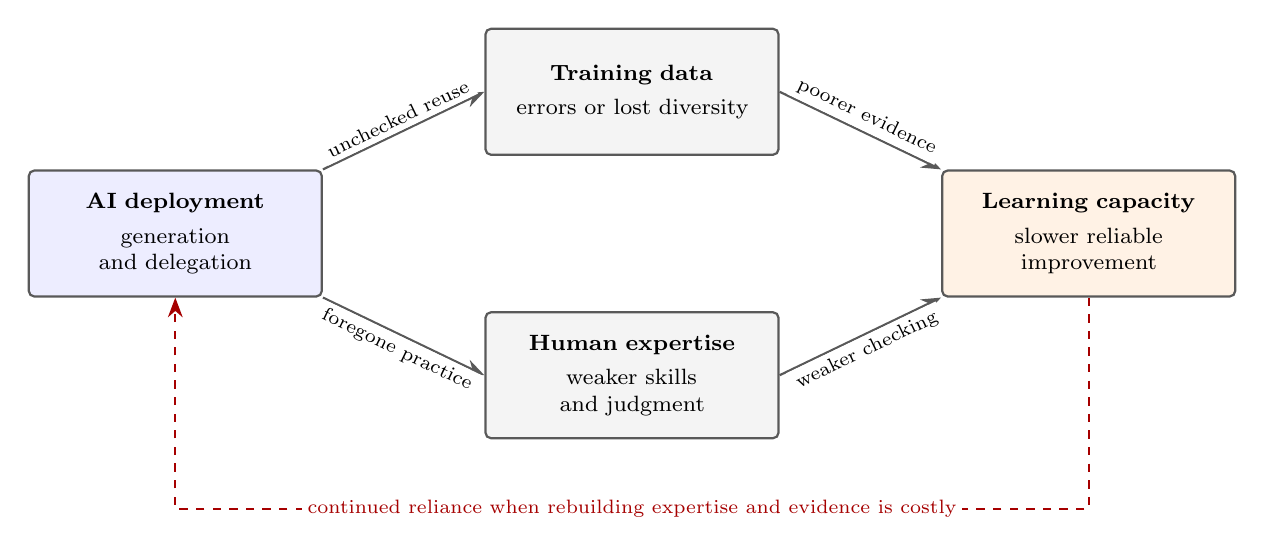
\begin{tikzpicture}[
  box/.style={draw=black!65, rounded corners=2pt, thick, align=center,
              text width=3.3cm, minimum height=1.6cm, inner sep=6pt,
              font=\footnotesize},
  arr/.style={-{Stealth[length=2.5mm]}, thick, draw=black!65},
  lbl/.style={font=\scriptsize, align=center, fill=white, inner sep=2pt},
]
\node[box, fill=blue!7] (A) at (0,0)
  {\textbf{AI deployment}\\[3pt]
   generation and delegation};
\node[box, fill=gray!9] (D) at (5.8,1.8)
  {\textbf{Training data}\\[3pt]
   errors or lost diversity};
\node[box, fill=gray!9] (H) at (5.8,-1.8)
  {\textbf{Human expertise}\\[3pt]
   weaker skills and judgment};
\node[box, fill=orange!10] (L) at (11.6,0)
  {\textbf{Learning capacity}\\[3pt]
   slower reliable improvement};
\draw[arr] (A.north east) -- (D.west)
  node[lbl, midway, above, sloped] {unchecked reuse};
\draw[arr] (A.south east) -- (H.west)
  node[lbl, midway, below, sloped] {foregone practice};
\draw[arr] (D.east) -- (L.north west)
  node[lbl, midway, above, sloped] {poorer evidence};
\draw[arr] (H.east) -- (L.south west)
  node[lbl, midway, below, sloped] {weaker checking};
\draw[arr, dashed, draw=red!65!black]
  (L.south) -- (11.6,-3.5) -- (0,-3.5) -- (A.south);
\node[lbl, text=red!65!black] at (5.8,-3.5)
  {continued reliance when rebuilding expertise and evidence is costly};
\end{tikzpicture}}
\caption{The Middle-Intelligence Trap: two conditional feedback channels.
Unchecked reuse can weaken training data, and displaced practice can
weaken expertise. The dashed return path requires costly adjustment or
unpriced spillovers. Verification, independent evidence, and replacement
training can interrupt the loop.}
\label{fig:trap}
\end{figure}

The collective channel runs through the training data. Externally evaluated generation can
improve training data; poorly selected recursive output can instead
propagate errors or narrow coverage. Our broader hypothesis is that
systems relying heavily on inherited records may also favor familiar
problem framings. This does not follow from distributional support
alone. If machine systems become reliable sources of new framings and
independent evaluation, this channel weakens. Survey evidence is
suggestive rather than decisive: 49 percent of scientists report that
AI steers them toward safer, more incremental projects, compared with
28 percent who report greater willingness to pursue risky questions
\citep{CodreanuEtAl2026AIScience}. These perceptions do not establish
changes in scientific novelty.

The individual channel runs through human expertise. Delegating a task can reduce practice
in the skills used to perform it, while also freeing time for other
forms of learning. Cognitive offloading therefore has an ambiguous
effect on net capability \citep{RiskoGilbert2016}. Skill loss is a
concern when the delegated activity is itself an important source of
training and no substitute practice occurs. Evidence specific to
generative AI remains limited. A survey associates heavier AI reliance
with weaker critical-thinking performance \citep{Gerlich2025}; it does
not establish long-run deterioration in professional judgment.
The employment pattern for workers aged 22--25 reviewed in
Section~\ref{subsec:deployment-skew} raises a related question: if junior
tasks provide training for future evaluators, how is that training
replaced when those tasks are delegated? The age pattern itself does not
measure changes in expertise.

The channels may reinforce one another. Weaker judgment can mean
less checking and less independent evidence, limiting the quality of
later training. As generated explanations become cheaper,
\emph{meta-explanation}---the capacity to question, calibrate, and
cross-validate them---may become more valuable. This loop can also be
constructive: effective verification and new evidence allow generated
output to improve the record.

\paragraph{When verification has an external benefit.}
Checking current output improves future training only if a corrected
output or informative evaluation reaches that training process. A firm
that checks an answer internally but releases the original version need
not improve the shared corpus. A provider that captures corrections
through its own service may internalize some of their value. An
externality arises when useful corrections are transmitted and part of
the resulting benefit accrues beyond the decision maker who pays for
them.

Proposition~\ref{prop:underprovision} formalizes a benchmark in which
verification improves a shared data stock and each adopter treats the
future benefit as external. The resulting private incentive to check is
too low. Transmission and appropriation determine how closely a
particular market resembles that benchmark. Rights to corrected data,
provenance, feedback contracts, and compensation for evaluation can
change both margins. Integration may internalize a benefit while also
increasing market power. The policy question is therefore which
institutional arrangement sustains valuable checking and broad access
to its benefits, rather than whether more checking is always desirable.

\paragraph{What could make the problem persist?}
A bottleneck can induce investment; a trap requires reasons why that
response remains inadequate. Three candidate mechanisms deserve
attention. First, dispersed benefits can weaken incentives to maintain
shared evidence even when its social value is high. Second, skill
formation is slow: a firm can hire an experienced evaluator today while
having little incentive to finance training whose benefits may accrue
to future employers. If many firms make that choice, replenishing the
pool of expertise becomes more costly. Third, once sources are difficult
to distinguish and alternatives have weakened, obtaining independent
evidence may require expensive new measurement or experimentation.

These mechanisms could reinforce reliance on the current system while
making recovery progressively more costly. They could also be offset
by better training technology, verification services, or contracts that
internalize future returns. Evidence of errors or reduced practice is
therefore insufficient to establish a trap. One must also show that
corrective investment fails to restore learning capacity over the
relevant horizon. The model in Appendix~\ref{app:model} establishes a
verification wedge under stated assumptions; a persistent trap would
require additional dynamics for expertise, data selection, and the
investment response.

\paragraph{Escaping the trap.}
Four possible responses merit economic evaluation. \emph{Cognitive
reserves}, or deliberate unassisted practice, raise questions about
which professional skills depreciate under delegation and how quickly.
\emph{Strategic friction} requires engagement at judgment points,
creating a trade-off between learning or verification and immediate
convenience. Its design raises the question of where to require such
engagement and when its private and external benefits justify the
costs imposed on users. \emph{Evaluation} in schools, journals, and
firms that rewards reasoning and meta-explanation as well as output
may strengthen incentives to develop and apply evaluative judgment. Finally,
\emph{economics education} can prepare graduates for this division of
labor.

Proposition~\ref{prop:underprovision} identifies a potential rationale
for intervention when corrections benefit a shared training corpus.
It does not establish the effectiveness of these responses or rank them
against standards, liability, or provenance requirements. Their benefits
must be assessed against implementation costs and effects on access,
innovation, and learning.

\paragraph{Economic questions.}
How fast do professional skills depreciate under delegation, and who
finances apprenticeship when its tasks can be automated? Which contracts
reward corrections that benefit other users, and when does a temporary
verification bottleneck become a persistent constraint on learning?

% =====================================================================
% Section 6 -- Concluding Remarks
% =====================================================================
\section{Concluding Remarks}\label{sec:conclusion}

This survey has connected AI's methodological and economic roles
through intelligence as a produced factor: produced from data and
compute, supplied separately from human labor, costly to check and
direct, and partly fed by its own output. Three lessons follow.

First, machine learning has an established role in prediction,
measurement, and computational approximation. Economists remain
responsible for identification, economic structure, objective
specification, and validation. The reason is illustrated by
\citet{Lucas1976}: predictive relationships need not remain invariant
when policy changes incentives and expectations. Similarly, fitting a
corpus does not by itself identify the mechanisms behind its records.
LLM-based measurement and simulated subjects add concerns about
coverage, correlated errors, and external validity. Further progress
requires methods for validating these tools and training economists to
use them.

Second, evidence on the economic consequences is less mature. Task
experiments do not settle aggregate employment effects, and one U.S.
payroll study finds relative declines concentrated among workers aged
22--25. Our deployment evidence identifies a further margin:
concentration on an occupation's core tasks is conditionally correlated
with lower employment growth in the retained CPS sample. Market structure
also remains unsettled. Large fixed costs and data feedback coexist
with relatively low raw-API switching costs and potentially substantial
integration costs. Comparative governance research should likewise
consider the Chinese record of platform enforcement and algorithm
regulation alongside the European Union's risk-based statute and the
U.S. federal sectoral approach.

Third, cheaper generation can shift scarcity toward verification and
direction. These complements affect both current output and future
capability: corrections may improve subsequent training, while
delegation changes opportunities to develop evaluative expertise. The
Middle-Intelligence Trap is the hypothesis that adverse feedback
between these channels can persist when corrective investment is
inadequate. Proposition~\ref{prop:underprovision} establishes a
verification externality when corrections reach a shared corpus and
their benefits are not fully internalized. It does not establish the
broader trap or require an absolute human--machine boundary.

The four questions of Section~\ref{sec:open} define three research
agendas: measuring useful cognitive services and their deployment within
occupations; modeling growth and market structure when training-data
quality is endogenous; and evaluating institutions that sustain
verification, independent evidence, and the formation of expertise.
The deployment evidence is a first contribution to the measurement
agenda. The formal framework identifies one incentive problem for the
theoretical and institutional work that remains.

\printbibliography

% =====================================================================
% Appendices
% =====================================================================
\appendix
\counterwithin{table}{section}
\section{Model Details}\label{app:model}

This appendix presents a stylized framework for
Section~\ref{sec:open}; it is deliberately compact, and each block
formalizes one strand of the text. The task technology and the
scaling-law cost of precision underpin
Section~\ref{subsec:tokenization}'s reading of intelligence as a
produced factor; the adoption frontier motivates the within-occupation
reading of the deployment evidence of
Section~\ref{subsec:deployment-skew}; and the verification choice
introduced into the adoption decision carries
Section~\ref{subsec:scarcity}'s bottleneck and, through the quality of
the corpus it leaves behind, the self-reproduction loop and the
verification externality of Section~\ref{subsec:trap}.

The model orders tasks by required precision, whereas the empirical
index ranks them by O*NET importance and relevance. No mapping between
these rankings is imposed. The model therefore motivates studying
deployment within occupations but does not derive the sign of the
employment association in Table~\ref{tab:aap}.

\paragraph{Task technology.}
Final output aggregates tasks indexed by $i \in [0,1]$ and ordered by the
precision their execution requires. Each task combines physical capital $k_i$,
non-cognitive labor $\ell_i$, and a cognitive input $H_i$ that itself
nests human cognition $h_i$ and AI inference services $m_i$ in constant
elasticity form:
\begin{equation}\label{eq:tasktech}
y_i = A_i\, k_i^{\alpha_i}\, \ell_i^{\beta_i}\,
      H_i^{\,1-\alpha_i-\beta_i},
\qquad
H_i = \Big[ \varphi_i\, h_i^{\frac{\sigma_i-1}{\sigma_i}}
      + (1-\varphi_i)\,\big(\theta_i(\psi_t)\, m_i\big)^{\frac{\sigma_i-1}{\sigma_i}}
      \Big]^{\frac{\sigma_i}{\sigma_i-1}},
\end{equation}
where $\theta_i(\psi_t)$ is task-specific AI quality, rising in the
frontier capability index $\psi_t$, and $\sigma_i$ is the elasticity of
substitution between human and machine cognition. We impose $A_i>0$,
$k_i,\ell_i,h_i,m_i\ge0$ (using the continuous extension at zero),
$0\le\alpha_i,\beta_i$, $\alpha_i+\beta_i<1$, $0<\varphi_i<1$,
$\theta_i(\psi_t)>0$, and $\sigma_i>0$; equation
\eqref{eq:tasktech} is read in its Cobb--Douglas limit when $\sigma_i=1$.
The parameter $\sigma_i$ governs substitution within the cognitive
aggregate, while $\theta_i(\psi_t)$ shifts the relative efficiency of AI.
The effect of improved AI on human labor demand also depends on relative
prices, output demand, and adjustment elsewhere in the economy.

\paragraph{The scaling-law cost of precision.}
The supply side is a stylized, task-level version of empirical scaling
laws, which relate a model's attainable loss to its size, training data,
and compute \citep{Kaplan2020}.

\begin{assumption}[Scaling-law cost of precision]\label{ass:scaling}
Adapting a frontier model of capability $\psi_t\ge0$ to task $i$ with
task-specific compute $C>0$ and data $D>0$ attains the error
\begin{equation}\label{eq:scaling}
\varepsilon_i \;\approx\; a_i(\psi_t)\, C^{-\gamma_i}\, D^{-\delta_i}
              + \varepsilon_i^{\min},
\qquad \gamma_i, \delta_i > 0,\quad a_i > 0,\quad a_i' < 0,
\end{equation}
with $\varepsilon_i^{\min}\!\ge 0$ a task-specific error floor: a more
capable frontier model needs less task-specific compute and data to
reach a given error.
\end{assumption}

Throughout, $P_c,P_d>0$ and
$\varepsilon_i^{\mathrm{req}}>\varepsilon_i^{\min}$. Under
Assumption~\ref{ass:scaling}, minimizing the outlay $P_c C + P_d D$
subject to the scaling relation in \eqref{eq:scaling}, treated as an
equality in this stylized model,
gives the cost of reaching a target error $\varepsilon$,
\begin{equation}\label{eq:precisioncost}
K_i(\varepsilon;\psi_t,P_c,P_d)
= (\gamma_i+\delta_i)
  \left[\frac{a_i(\psi_t)}{\varepsilon-\varepsilon_i^{\min}}
  \Big(\frac{P_c}{\gamma_i}\Big)^{\gamma_i}
  \Big(\frac{P_d}{\delta_i}\Big)^{\delta_i}
  \right]^{\frac{1}{\gamma_i+\delta_i}},
\end{equation}
which is decreasing and convex in the target error, diverges as
$\varepsilon \downarrow \varepsilon_i^{\min}$, rises in both prices, and
falls in capability. The outlay needed to reach task $i$'s required
precision $\varepsilon_i^{\mathrm{req}}$ at date $t$ is therefore
\begin{equation}\label{eq:upfront}
C_i^{\mathrm{upfront}}(t)
= K_i\big(\varepsilon_i^{\mathrm{req}};\psi_t,P_c(t),P_d(t)\big)
+ J_i^{\mathrm{inst}}(t),
\end{equation}
where $P_c$ and $P_d$ price compute and data and $J_i^{\mathrm{inst}}$ is
an institutional wedge collecting integration, compliance, and
workflow-redesign costs. Equation~\eqref{eq:upfront} implies that marginal precision becomes
more expensive near the error floor. It does not characterize the
optimization landscape of neural-network training. The framework prices capability as
this upfront outlay plus a constant inference price $p_t$;
test-time-compute pricing, under which additional inference outlay buys
additional precision on a given task, would make $\varepsilon_i$ depend
on the inference budget as well, a natural extension we leave aside.

\paragraph{Endogenous adoption.}
Automation is an investment decision. With human wage $w_i$, inference
price $p_t$, task volume $\mathrm{Scale}_i$, and discount rate $\rho$,
the adopter also chooses a verification intensity $e_i \in [0,1]$, the
share of machine output that is checked, at per-unit cost
$v_i:[0,1]\to\mathbb R_+$
with $v_i(0)=0$, $v_i' > 0$, $v_i'' > 0$; an unchecked unit that is wrong costs
the adopter $\kappa_i$, and errors occur with probability
$\pi_i(\psi_t)$, falling in capability. The benchmark assumes that
checking detects and corrects errors in checked units, with correction
costs included in $v_i$. We take
$w_i,p_t,\kappa_i,J_i^{\mathrm{inst}}\ge0$,
$\mathrm{Scale}_i,\rho>0$, and $\pi_i(\psi_t)\in[0,1]$. The present value of
substituting machine for human cognition, at current prices, is
\begin{equation}\label{eq:value}
V_i(t) = \max_{e_i \in [0,1]}\,
         \big(w_i - p_t - v_i(e_i)
         - (1-e_i)\,\pi_i(\psi_t)\,\kappa_i\big)\,
         \mathrm{Scale}_i/\rho,
\end{equation}
and task $i$ is automated at $t$ when
$V_i(t) \ge C_i^{\mathrm{upfront}}(t)$, a net-present-value rule that
leaves aside the option to wait for cheaper adoption. Let
$\mathcal A_t=\{i:V_i(t)\ge C_i^{\mathrm{upfront}}(t)\}$. When this set
is nonempty, its frontier is $i^{*}(t)=\sup\mathcal A_t$; when it is
empty, automated mass and deployment are defined as zero and statements
involving $i^*$ apply only after adoption begins.
The private verification choice solves
$v_i'(e_i^{p}) = \pi_i(\psi_t)\,\kappa_i$ at an interior optimum: the
adopter checks until the marginal cost of checking equals the expected
marginal loss avoided.
The verification term incorporates Section~\ref{subsec:scarcity}'s
bottleneck: holding other costs and benefits fixed, higher checking
costs or larger losses from undetected errors reduce the net value of
automation, even when inference is inexpensive. Equation~\eqref{eq:value} is a separate full-replacement benchmark:
$w_i$ and $p_t$ are costs per equivalent unit of task service, with
productivity and CES weights absorbed into the units. Perfect
substitutability alone does not remove those adjustments from
equation~\eqref{eq:tasktech}. With finite elasticity, adoption requires
solving the cost-minimization problem within $H_i$; the results below
apply to that extension only if its net adoption value satisfies the
stated monotonicity and single-crossing conditions.

\begin{remark}[So-so automation]\label{rem:soso}
An adopter who prices the machine at $w_i - p_t$ and ignores both the
verification cost and the cost of undetected error (sets $e_i = 0$ and
$\kappa_i = 0$ in its accounts) automates every task with
$(w_i - p_t)\,\mathrm{Scale}_i/\rho \ge C_i^{\mathrm{upfront}}$,
including tasks whose true value \eqref{eq:value} falls short of that
outlay.
The adopter's accounts can therefore overstate the net gain. If
others bear the checking costs, those costs are also omitted. This is the
verification-cost version of the so-so-automation pattern of
\citet{AcemogluRestrepo2019NewTasks}.
\end{remark}

\begin{proposition}[The adoption frontier and the S-curve]\label{prop:scurve}
Index tasks so that required precision tightens with $i$, and suppose
that the net value of automation,
$N_i(t) = V_i(t) - C_i^{\mathrm{upfront}}(t)$, is continuous and strictly
decreasing in $i$ (single crossing). Then (i) the
automated set is empty or an interval $[0, i^{*}(t)]$, so that tasks are
automated in the order in which they are indexed. (ii) For parameter
changes under which single crossing continues to hold, the frontier $i^{*}(t)$ is
non-decreasing in capability $\psi_t$ and non-increasing in the prices
$P_c(t)$, $P_d(t)$, and $p_t$,
in an upward shift of the institutional wedge $J^{\mathrm{inst}}$, and in an
upward shift of the verification cost schedule $v(\cdot)$ or of
$\kappa$. (iii) Suppose that, for every finite capability and finite
strictly positive price vector,
$K_i(\varepsilon_i^{\mathrm{req}};\psi_t,P_c,P_d)\to\infty$ as
$i\to1$, uniformly on compact sets of those arguments, while
$V_i(t)$ remains bounded. Then $i^{*}(t)<1$ at every finite date: a tail
of high-precision tasks is not automated. (iv) Let $\mu(i)>0$ be a
continuous value-weighted density of tasks and
$M(t) = \int_0^{i^{*}(t)} \mu(i)\,\mathrm{d}i$ the automated mass, to
which cumulative productivity gains are proportional when saving per
unit of task value is constant. After adoption begins, suppose
$i^*(t)$ is differentiable, $i^*(t)\to0$ at the initial endpoint,
$i^*(t)\to\bar i<1$ in the long run, and
$\dot M(t)=\mu(i^*(t))\dot i^*(t)$ is nonnegative, tends to zero at
both endpoints, and rises to a single peak before falling (as when
$\mu$ is single-peaked and the frontier advances at a constant speed
until it stops at $\bar i$). Then $M(t)$
is S-shaped and converges to the capped plateau
$\int_0^{\bar i}\mu(i)\,\mathrm{d}i$.
\end{proposition}

\begin{proof}[Proof sketch]
With $N_i(t)$ strictly decreasing in $i$, the set
$\{\,i : N_i(t) \ge 0\,\}$ is an interval starting at zero (empty if
$N_0(t) < 0$), which gives (i) without assigning a supremum to the empty
set, and any change that raises $N_i(t)$ at
every $i$ moves its upper end weakly outward. For (ii), $K_i$ in
\eqref{eq:precisioncost} falls in $\psi_t$ and rises in $P_c$ and $P_d$,
and by the envelope theorem $V_i$ in \eqref{eq:value} rises as
$\pi_i(\psi_t)$ falls and falls in $p_t$, in $\kappa$, and in upward
shifts of $v(\cdot)$. Data act through capability: a larger effective
stock raises $\psi_t$ by \eqref{eq:psidot} below. For (iii), bounded
$V_i$ minus a uniformly diverging $K_i$ is negative near $i=1$. For
(iv), the fundamental theorem of calculus gives
$\dot M=\mu(i^*)\dot i^*$. The assumptions on this product make $M$
first convex and then concave, with a horizontal long-run limit;
convergence of $i^*$ gives the displayed plateau. A single-peaked task
density alone does not guarantee these conditions, because the speed
and stopping point of the frontier also matter. Single crossing is assumed, not
derived: the convexity of $K_i$ makes cost rise ever more steeply as
precision tightens while value stays bounded, which makes the condition
natural, but it does not follow without restrictions on how wages,
scale, and the scaling parameters vary across tasks. The shape is a
characterization under the stated conditions, not a theorem free of them.
\end{proof}

Proposition~\ref{prop:scurve} therefore separates the interval and
comparative-static results from the additional endpoint restrictions
needed for a capped S-curve.

\paragraph{Dynamics and self-reproduction.}
What separates the framework from a static automation model is a feedback
loop. Frontier capability accumulates as
\begin{equation}\label{eq:psidot}
\dot{\psi} \;=\; \eta(\psi)\; I_{\mathrm{compute}}(t)\; D_{\mathrm{eff},t},
\qquad \eta > 0,\quad \eta'(\psi) < 0,
\end{equation}
where $I_{\mathrm{compute}}$ is training investment and $\eta$ is a
declining learning efficiency; take $I_{\mathrm{compute}}\ge0$ and all
data stocks nonnegative, with $D_{\mathrm{total},t}>0$. Data supply is partly endogenous:
deployed AI manufactures training material,
$D_{\mathrm{total},t} = D_{\mathrm{human},t} +
D_{\mathrm{synthetic}}(\psi_t,E_t)+
D_{\mathrm{scored}}(\psi_t,E_t)$, where $E_t$ is the mass of
$\mathcal A_t$ (zero when that set is empty). The deployment channel is
explicitly
$D_{\mathrm{synthetic},E},D_{\mathrm{scored},E}\ge0$; we also maintain
$D_{\mathrm{synthetic},\psi},D_{\mathrm{scored},\psi}\ge0$ when greater
capability itself raises generated-data volume. Let
$s_t=D_{\mathrm{synthetic}}/D_{\mathrm{total},t}$ be the share of
open-ended synthetic data and
$z_t=D_{\mathrm{scored}}/D_{\mathrm{total},t}$ the share of generated
data evaluated by an external rule. Under the single-crossing condition, and when $\mathcal A_t$ has
positive mass, let
$\bar{e}_t = \int_0^{i^{*}(t)} \omega_i\, e_i\,\mathrm{d}i$ be the
average verification intensity on automated tasks, weighted by volume,
$\omega_i = \mathrm{Scale}_i \big/ \int_0^{i^{*}(t)}
\mathrm{Scale}_j\,\mathrm{d}j$; set $\bar e_t=0$ when the automated set has zero mass.
Effective data are discounted for
quality,
\begin{equation}\label{eq:quality}
D_{\mathrm{eff},t} = q(\bar{e}_t,s_t,z_t)\,D_{\mathrm{total},t},
\qquad q\in(0,1],\quad q_e>0,\quad q_{ee}\le0,\quad q_s\le0,\quad q_z\ge0,
\end{equation}
where $q_s<0$ only when open-ended synthetic observations displace or
sufficiently dilute independent real data; $q_s=0$ permits benign
accumulation. The $z_t$ channel permits externally scored generation to
add information. Verification reduces contamination in this reduced-form specification;
it need not restore information absent from the original sample. The
benchmark assumes that checked outputs or their corrections reach the
training corpus and improve its quality. Internal review with no
transmission to training does not satisfy this assumption. Under the derivative restrictions above, capability can
raise deployment, deployment generates data, and data feed back into
capability through \eqref{eq:psidot}.

Two mechanisms sit behind \eqref{eq:quality}, and they are not
equivalent. The synthetic share $s_t$ captures \emph{information
recycling}: sampling from a fitted model need not add independent
evidence about the target distribution. Under some recursive training
procedures, approximation and sampling errors progressively erode the
representation of rare cases \citep{Shumailov2024}. The outcome depends
on whether synthetic data replace real data or accumulate alongside
them \citep{AlemohammadEtAl2024MAD, GerstgrasserEtAl2024Accumulate};
related analyses find changes in scaling laws
\citep{DohmatobEtAl2024Tails}.
Recycling is one possible source of lost learning value, even when
individual synthetic units are correct. Externally evaluated generation,
such as self-play scored by the rules of Go
(Section~\ref{subsec:tokenization}), can instead add useful training
information through $z_t$. Benign accumulation can likewise
have $q_s=0$; the strict $q_s<0$ case is reserved for displacement or
sufficient dilution. Verification $\bar{e}_t$ addresses \emph{contamination}: the benchmark
assumes that checking detects and corrects some errors before they
enter the corpus. Loss of
\emph{provenance} is not a third term but can make later filtering more
difficult: when source information is unavailable, generated output
cannot be reliably separated by origin, which is why provenance
requirements appear among the institutional responses of
Section~\ref{subsec:trap}. The quality discount therefore differs from
the depreciation of data in \citet{FarboodiVeldkamp2021DataEconomy},
where old data lose value because the state they describe has moved on;
here the state is fixed, and it is the composition of the corpus that
changes.

The dynamics depend on the paths of training investment, data supply,
and data quality, as well as declining learning efficiency
$\eta(\psi)$. The precision-cost
schedule separately limits adoption near task-specific error floors.
These mechanisms can moderate growth, but the restrictions given here
do not imply a bounded capability path or select among stagnation,
sustained growth, and accelerating growth. In particular,
equation~\eqref{eq:psidot} permits slower accumulation but no decline in
the capability stock. A model of a self-sustaining trap would also need
a law of motion for human judgment and further restrictions on data and
investment dynamics.

\begin{proposition}[Private underprovision of verification]\label{prop:underprovision}
Suppose the automated set has positive mass and
$I_{\mathrm{compute}}(t)>0$. Each adopter is small, receives no compensation for improving the
shared training corpus, takes $\bar{e}_t$ and hence
$q(\bar{e}_t,s_t,z_t)$
as given, and chooses $e_i^{\,p}$ with
$v_i'(e_i^{\,p}) = \pi_i(\psi_t)\,\kappa_i$. A planner who bears the same
direct costs, attaches a shadow value $\lambda_t > 0$ to capability, and
chooses verification on the automated tasks at date $t$ also counts the
effect of $e_i$ on $\bar{e}_t$ and hence
on $\dot{\psi}$ through \eqref{eq:psidot}--\eqref{eq:quality}. At an
interior optimum,
\begin{equation}\label{eq:wedge}
v_i'(e_i^{\,s}) = \pi_i(\psi_t)\,\kappa_i + \tau_t,
\qquad
\tau_t = \frac{\lambda_t\,\eta(\psi_t)\, I_{\mathrm{compute}}(t)\,
         q_e(\bar{e}_t,s_t,z_t)\, D_{\mathrm{total},t}}
        {\int_0^{i^{*}(t)} \mathrm{Scale}_j\,\mathrm{d}j} \;>\; 0,
\end{equation}
so that $e_i^{\,p} < e_i^{\,s}$ on every automated task with an interior
solution:
verification is underprovided relative to the social optimum. The wedge
$\tau_t$ is the same on every task: it is the value of the data quality
that checking one more unit of machine output preserves. Holding the other terms fixed, the wedge is larger when data quality
is more sensitive to checking ($q_e$). It is weakly increasing in the
synthetic share through this channel if $q_{es} \ge 0$. If training
investment is zero, this contemporaneous wedge is zero and strict
underprovision does not follow. This is the verification externality of Section~\ref{subsec:trap}.
Its existence depends on transmission to a shared corpus and benefits
that the adopter does not capture; technical evidence of model collapse
alone does not establish those institutional conditions.
\end{proposition}

\begin{proof}[Proof sketch]
The planner's objective at date $t$ is the flow surplus on automated
tasks,
$\int_0^{i^{*}(t)} \big(w_i - p_t - v_i(e_i)
- (1-e_i)\,\pi_i(\psi_t)\,\kappa_i\big)\,\mathrm{Scale}_i\,\mathrm{d}i$,
plus $\lambda_t\,\dot{\psi}$; $\lambda_t>0$ is the assumed shadow value of capability, whose benefits
include lower error rates and adoption costs. Differentiating with respect to
$e_i$, with $\partial \bar{e}_t/\partial e_i = \omega_i$, and dividing by
$\mathrm{Scale}_i$ gives \eqref{eq:wedge}. Because $v_i'$ is strictly
increasing and $\tau_t > 0$, $e_i^{\,s} > e_i^{\,p}$, and the gap rises
with $\tau_t$. The objective is concave in the $e_i$ ($v_i'' > 0$,
$q_{ee} \le 0$), so the first-order conditions are sufficient. The
planner takes the automated set as given; the effect of verification on
adoption itself is left aside.
\end{proof}


\paragraph{Transmission and appropriation.}
The benchmark separates private losses from a shared benefit of
verification. To see how transmission matters, let $\chi_i\in[0,1]$
measure the fraction of task $i$'s checking whose useful corrections
reach training. Replacing $\bar e_t$ in the quality function with
$\bar r_t=\int_0^{i^*(t)}\omega_i\chi_i e_i\,\mathrm{d}i$ makes the
planner's additional marginal benefit on task $i$ equal to
$\chi_i\tau_t$, with $q_e$ in \eqref{eq:wedge} replaced by $q_r$.
The same differentiation yields this result for fixed transmission
rates. When $\chi_i=0$, private checking has no benefit through this
channel. Feedback contracts or ownership arrangements that allow an
adopter to capture part of that benefit can narrow the incentive gap;
modeling their equilibrium design would require specifying rights,
payments, and bargaining. The uniform wedge in
Proposition~\ref{prop:underprovision} is thus the full-transmission,
uncompensated benchmark, not a claim about every deployment.

\section{Data, Sample, and Robustness for the Deployment-Skew Evidence}\label{app:evidence}

\paragraph{Data.}
\emph{AI usage} comes from the March 2026 release of the Anthropic
Economic Index \citep{MassenkoffEtAl2026AEI}: one million conversations
on the Claude.ai Free, Pro, and Max plans from 5 to 12 February 2026.\footnote{%
Release documentation:
\href{https://huggingface.co/datasets/Anthropic/EconomicIndex/blob/main/release_2026_03_24/data_documentation.md}{March 2026};
\href{https://huggingface.co/datasets/Anthropic/EconomicIndex/blob/main/release_2026_06_26/data_documentation.md}{June 2026}.}
A privacy-preserving pipeline assigns each classified conversation to a single O*NET
task statement, and the smallest task
reported has 15 conversations. The release lists 3,258 task statements
with their shares of all conversations; another 7 percent of
conversations are unassigned or unclassified. Because every
share is a fraction of the same pool, usage is on a common scale across
occupations, which a share computed within each occupation would not be.
The measure has four limits: it counts conversations, not hours or
value; it observes one assistant family, whose users skew technical; it
places each conversation on a single task; and it classifies
conversations by task, not by the occupation of the user. The March 2026 release is
the latest that can be used: the June 2026 release rounds task shares to
two decimal places, too coarse for a within-occupation curve when the
median task share is 0.005 percent. The March 2025 release,\footnote{%
Anthropic, \emph{The Anthropic Economic Index}, release of 27 March
2025, \url{https://www.anthropic.com/economic-index}.} one million
conversations on the Free
and Pro plans from the 11 days after the launch of Claude 3.7 Sonnet,
serves as a check. \emph{Task structure} comes from O*NET 27.2
\citep{ONET272}. The rated analytical file contains 17,953
occupation--task pairs in 873 occupations
for importance (on a scale of 1 to 5) and relevance (the percentage of
incumbents who report the task).

\emph{Household employment} comes from the CPS basic monthly files, accessed through IPUMS
\citep{IPUMSCPS2025}: employed persons aged 22 to 55, weighted by final
person weights and aggregated to 2018 Census occupation codes. The
demographic controls are shares of survey respondents in each
occupation, not weighted by the person weights. The
baseline averages each occupation's monthly share of employment over
January 2019 to October 2022 and over November 2022 to March 2026. October
2025 is missing, because household-survey data were not collected during
the lapse in federal appropriations, so the second period has 40 months.
The CPS adopted the 2018 codes in January 2020, and the monthly panel uses
2019 records only where the 2010 code coincides with a 2018 code, so for
71 of the 253 occupations the first average starts in January 2020. The
histories of nine additional occupations cover only part of 2019. The
point-year windows use a separate extract of annual averages for 2019,
2021, 2022, and 2025 (1,554,086 person-month records), in which 2019
records are converted with the Census Bureau crosswalk and codes
identical in the two schemes are carried over, placing 92 percent of
2019 records (94 million workers, against 114 million in the monthly
panel). \emph{Payroll employment} comes from the national OEWS
estimates for detailed occupations in May 2019 and May 2025
\citep{BLSOEWS}. Finally, O*NET occupations map to SOC codes by dropping
the O*NET suffix, and SOC codes map to Census codes through the Census
Bureau's code list \citep{CensusOcc2018}. The list gives each Census code
a detailed SOC code, a broad code (such as 11-2030), or a wildcard for a
residual group (such as 13-20XX, ``Other financial specialists''). Broad
codes take all their detailed members, and wildcards take the members not
listed under another code.

\paragraph{Indices.}
Equations~\eqref{eq:skew} and \eqref{eq:intensity} define the two
indices. Tasks are ordered by the weight
$w_j=\mathrm{IM}_j\cdot(\mathrm{RT}_j/100)$,
and the two normalizations in equation~\eqref{eq:coords} do different
jobs. Dividing the horizontal axis by $\sum_j w_j$ expresses position as a
share of total task weight. This removes the overall scale of the
weights, but the measure can still depend on how O*NET divides work
into task statements. Dividing the vertical axis by $\sum_j c_j$
makes every curve end at $(1,1)$ whatever the occupation's total usage,
which strips the level out of $G$. The level is relocated into $\bar{U}$,
which weights by importance alone rather than by $w_j$ and averages over
all rated tasks, those without usage included, so that level and shape
are built from different features of the data. The regressions use $u$,
the standardized logarithm of $\bar{U}$, because in levels a handful of
occupations dominate: the heaviest user lies more than nine standard
deviations above the mean. The control $f_{\mathrm{eff}}=1/(N H)$, where
$N$ is the number of tasks and $H$ the Herfindahl index of the
contribution shares $c_j/\sum_k c_k$, is the effective fraction of tasks
drawing usage.

For $G$, each occupation's piecewise-linear concentration curve is
interpolated on the 101-point grid
$\{0,0.01,\ldots,1\}$ and integrated by the trapezoid rule.

$G$ is computed only for occupations with usage on at least three tasks.
With usage on a single task, the piecewise-linear curve rises only
across that task's weight interval. If its endpoints are $x_{j-1}$ and
$x_j$, exact integration gives $G=1-x_{j-1}-x_j$; the grid-based
calculation approximates this value. The index then largely records
the location of one match. With only two matched tasks, it remains
highly sensitive to either match. All
indices are computed for each O*NET occupation and averaged to Census
codes with weights equal to the number of tasks, $G$ and
$f_{\mathrm{eff}}$ over the occupations that meet the three-task rule.
Within each estimation sample, $G$, $u$, and $f_{\mathrm{eff}}$ are
standardized; demographic shares enter as proportions. Core and
peripheral tilt are formed from the raw index before centering and
divided by its standard deviation, as defined in
Section~\ref{subsec:deployment-skew}.

\paragraph{Sample.}
Table~\ref{tab:funnel} traces the sample from the source files, and three
steps do most of the work. The first is the text match. The index
classifies conversations against its own copy of O*NET, on an older
taxonomy (19,530 task statements in 974 occupations), while the ratings
come from release 27.2, so usage is matched to rated tasks by their
normalized text. The match recovers 2,619 of the 3,258 tasks with usage,
and 69 percent of all conversations. The largest loss is software
development: 7.5 percent of all conversations fall on tasks listed under
the two older software-developer titles that have no rated counterpart,
and release 27.2 rates no tasks for the current software-developer
occupation. Because a task text can belong to several occupations, the
2,619 tasks attach to 3,277 occupation--task pairs. The second step is the
usage filter: 240 of the 873 rated occupations have no matched usage and
229 have usage on only one or two tasks, which leaves 404. The filter is
selective. It keeps 66 to 100 percent of the occupations in management,
business and finance, computing and mathematics, law, education, arts and
media, and office support (SOC major groups 11, 13, 15, 23, 25, 27, and
43), but only 4 to 14 percent in farming, construction, installation and
repair, production, and transportation (groups 45, 47, 49, 51, and 53).
The estimates therefore describe the AI-using range of the occupation
distribution. The third step is the crosswalk to the CPS. Of the 565
civilian Census codes, 530 contain at least one rated O*NET occupation.
The other 35 are 18 residual ``all other'' categories and 17 occupations
without ratings in release 27.2, most of them new or redefined in the
2018 SOC (software developers, financial and investment analysts, project
management specialists, emergency medical technicians, and paramedics
among them). Of the 530, 266 contain an occupation that meets the
three-task rule, and 253 of these are observed in the CPS both before and
after November 2022; the other 13 never appear in the monthly panel. The
2019-based window keeps 200 occupations because of the 2020 recoding. At
the SOC level used for the payroll check, 319 of the 354 codes that meet
the rule are published as detailed occupations in both years.

\begin{table}[t]
\centering\small
\caption{From Source Files to the Estimation Sample}
\label{tab:funnel}
\begin{tabular}{@{}llr@{}}
\toprule
Step & Unit & Count \\
\midrule
Tasks with recorded usage (Anthropic Economic Index) & Task & 3,258 \\
\quad matched by text to rated O*NET 27.2 tasks & Task & 2,619 \\
Rated occupation--task pairs (O*NET 27.2) & Pair & 17,953 \\
\quad with matched usage & Pair & 3,277 \\
Occupations with rated tasks & O*NET & 873 \\
\quad with matched usage on at least one task & O*NET & 633 \\
\quad with matched usage on at least three tasks & O*NET & 404 \\
Civilian occupation codes, 2018 Census list & Census & 565 \\
\quad containing at least one rated O*NET occupation & Census & 530 \\
\quad containing an occupation with usage on three tasks & Census & 266 \\
\quad observed in the CPS before and after November 2022 & Census & 253 \\
Point-year windows: 2021 or 2022 base; 2019 base & Census & 253; 200 \\
SOC codes with usage on three tasks (payroll check) & SOC & 354 \\
\quad published by OEWS in May 2019 and May 2025 & SOC & 319 \\
\bottomrule
\end{tabular}
\end{table}

\paragraph{Robustness.}
Table~\ref{tab:robust} reports the checks summarized in
Section~\ref{subsec:deployment-skew}. With 2022 or 2019 as the base year
the coefficient on $G$ is as large as in the baseline; the 2019 window
loses a fifth of the occupations to the 2020 recoding of CPS occupations
and is less precise. The split between core and peripheral tilt is less
stable: in these two windows neither half is significant on its own, and
peripheral tilt takes a positive sign. Dropping the employment weights, the fifteen computer
and mathematical occupations, or the 25 occupations with the heaviest
usage leaves it between $-0.021$ and $-0.028$ for the share outcome.
Omitting the controls other than usage gives $-0.029$, and adding the
model-rated potential exposure of \citet{EloundouEtAl2024} as a control
gives $-0.027$. The March 2025 release gives $-0.024$. Estimated
separately for seven groups of workers (men, women, college graduates,
workers without a degree, and three age groups) over the three point-year
windows, $G$ is negative in all 21 cells and significant at the 5 percent
level in 13 for the share outcome and 10 for log employment. Over
2021--2025 the share estimate is significant among women, college
graduates, and each age group, workers aged 22 to 25 included, but not
among men or workers without a degree.

The three-task rule matters, for the reason given above. Among all 387
occupations with any usage, which hold 84 percent of employment, the
coefficient on $G$ is small and insignificant. For the occupations with
usage on one or two tasks $G$ is close to an indicator of whether the
matched task is central, and among them, where usage is slight, a central
match goes with employment gains: the slope of $G$ at light usage is
positive in that sample and disappears once they are excluded. The slope
at heavy usage is negative and significant at every threshold, and core
tilt is negative at every threshold and significant at the 5 percent
level from two tasks up. Raising the minimum to five tasks leaves the main qualitative
conclusions unchanged.

The coefficient on $G$ is not statistically significant in the
pre-period checks
(Table~\ref{tab:placebo}). On the change in employment
share from 2019 to 2022 the coefficient on $G$ is $-0.013$, and from
2021 to 2022 it is $-0.004$, neither significant; splitting the
pre-period of the monthly panel at January 2021 gives $-0.007$. The
point estimates are negative, and the 2019 window is the noisy one, so
the placebo has limited power.

In payroll data the association does not appear. For the 319 SOC
occupations that meet the three-task rule and are published by the OEWS
in both years, the coefficient on $G$ is close to zero, and only the
usage level enters, with a negative sign ($-0.058$). The March 2025
release gives $-0.029$ for $G$ in the same data, significant at the 10
percent level. Two differences between the surveys bear on this contrast.
The CPS counts workers aged 22 to 55 by self-reported occupation and the
OEWS counts payroll jobs at all ages, so the 2019 CPS total is about 0.81
of the OEWS total; and the gap varies by occupation, with self-reported
manager and supervisor titles far above establishment counts (by a factor
of 4.7 for chief executives). The finding is so far confined to
household-survey employment.

\begin{table}[p]
\centering\footnotesize
\setlength{\tabcolsep}{5pt}
\caption{Robustness of the Direction Result}
\label{tab:robust}
\begin{tabular}{@{}lcccccc@{}}
\toprule
 & & & & \multicolumn{2}{c}{Slope of $G$} & \\
\cmidrule(lr){5-6}
 & $G$ & $G^{+}$ & $G^{-}$ & Light usage & Heavy usage & $N$ \\
\midrule
\multicolumn{7}{@{}l}{\emph{Panel A. Proportional change in employment share}}\\
CPS, 2022--2025 & $-0.029^{***}$ & $-0.026$ & $0.033$ & $-0.014$ & $-0.036^{***}$ & 253 \\
 & $(0.010)$ & $(0.020)$ & $(0.023)$ & $(0.014)$ & $(0.012)$ & \\
CPS, 2019--2025 & $-0.030^{**}$ & $-0.033$ & $0.024$ & $-0.005$ & $-0.040^{***}$ & 200 \\
 & $(0.014)$ & $(0.027)$ & $(0.043)$ & $(0.022)$ & $(0.013)$ & \\
Unweighted & $-0.028^{**}$ & $-0.077^{***}$ & $-0.041$ & $0.000$ & $-0.047^{***}$ & 253 \\
 & $(0.012)$ & $(0.022)$ & $(0.028)$ & $(0.016)$ & $(0.015)$ & \\
Without computer occupations & $-0.021^{***}$ & $-0.033^{**}$ & $0.002$ & $-0.002$ & $-0.028^{***}$ & 238 \\
 & $(0.007)$ & $(0.015)$ & $(0.021)$ & $(0.010)$ & $(0.007)$ & \\
Without top 25 by usage & $-0.023^{**}$ & $-0.044^{***}$ & $-0.014$ & $-0.004$ & $-0.034^{***}$ & 228 \\
 & $(0.009)$ & $(0.016)$ & $(0.022)$ & $(0.010)$ & $(0.012)$ & \\
One or more used tasks & $-0.006$ & $-0.023^{*}$ & $-0.015$ & $0.029^{***}$ & $-0.031^{***}$ & 387 \\
 & $(0.009)$ & $(0.014)$ & $(0.017)$ & $(0.008)$ & $(0.010)$ & \\
Two or more used tasks & $-0.017^{*}$ & $-0.044^{***}$ & $-0.017$ & $0.022^{**}$ & $-0.036^{***}$ & 308 \\
 & $(0.009)$ & $(0.017)$ & $(0.020)$ & $(0.010)$ & $(0.009)$ & \\
Five or more used tasks & $-0.027^{***}$ & $-0.042^{**}$ & $0.000$ & $0.002$ & $-0.040^{***}$ & 156 \\
 & $(0.009)$ & $(0.019)$ & $(0.024)$ & $(0.013)$ & $(0.010)$ & \\
March 2025 release & $-0.024^{**}$ & $-0.040^{**}$ & $-0.003$ & $0.004$ & $-0.041^{***}$ & 250 \\
 & $(0.010)$ & $(0.018)$ & $(0.030)$ & $(0.012)$ & $(0.014)$ & \\
Payroll (OEWS), 2019--2025 & $0.004$ & $-0.018$ & $-0.039$ & $0.040$ & $-0.010$ & 319 \\
 & $(0.016)$ & $(0.030)$ & $(0.036)$ & $(0.029)$ & $(0.018)$ & \\
\addlinespace
\multicolumn{7}{@{}l}{\emph{Panel B. Change in log employment}}\\
CPS, 2022--2025 & $-0.032^{***}$ & $-0.029$ & $0.036$ & $-0.017$ & $-0.039^{***}$ & 253 \\
 & $(0.011)$ & $(0.020)$ & $(0.025)$ & $(0.018)$ & $(0.012)$ & \\
CPS, 2019--2025 & $-0.031^{*}$ & $-0.035$ & $0.026$ & $0.005$ & $-0.048^{***}$ & 200 \\
 & $(0.017)$ & $(0.032)$ & $(0.049)$ & $(0.025)$ & $(0.014)$ & \\
Unweighted & $-0.026^{**}$ & $-0.076^{***}$ & $-0.044$ & $0.005$ & $-0.048^{***}$ & 253 \\
 & $(0.012)$ & $(0.022)$ & $(0.028)$ & $(0.016)$ & $(0.015)$ & \\
Without computer occupations & $-0.021^{***}$ & $-0.033^{**}$ & $0.000$ & $0.002$ & $-0.029^{***}$ & 238 \\
 & $(0.007)$ & $(0.015)$ & $(0.021)$ & $(0.010)$ & $(0.007)$ & \\
Without top 25 by usage & $-0.020^{**}$ & $-0.042^{***}$ & $-0.018$ & $-0.001$ & $-0.033^{***}$ & 228 \\
 & $(0.009)$ & $(0.016)$ & $(0.022)$ & $(0.010)$ & $(0.012)$ & \\
One or more used tasks & $-0.005$ & $-0.023^{*}$ & $-0.017$ & $0.031^{***}$ & $-0.031^{***}$ & 387 \\
 & $(0.009)$ & $(0.013)$ & $(0.017)$ & $(0.009)$ & $(0.009)$ & \\
Two or more used tasks & $-0.015$ & $-0.044^{***}$ & $-0.020$ & $0.026^{**}$ & $-0.036^{***}$ & 308 \\
 & $(0.009)$ & $(0.017)$ & $(0.021)$ & $(0.011)$ & $(0.009)$ & \\
Five or more used tasks & $-0.027^{***}$ & $-0.041^{**}$ & $0.001$ & $0.005$ & $-0.040^{***}$ & 156 \\
 & $(0.009)$ & $(0.018)$ & $(0.025)$ & $(0.013)$ & $(0.009)$ & \\
March 2025 release & $-0.024^{**}$ & $-0.038^{**}$ & $0.000$ & $0.006$ & $-0.041^{***}$ & 250 \\
 & $(0.010)$ & $(0.016)$ & $(0.029)$ & $(0.012)$ & $(0.014)$ & \\
Payroll (OEWS), 2019--2025 & $0.005$ & $-0.023$ & $-0.047$ & $0.041$ & $-0.010$ & 319 \\
 & $(0.015)$ & $(0.028)$ & $(0.034)$ & $(0.027)$ & $(0.019)$ & \\
\bottomrule
\end{tabular}

\smallskip
\begin{minipage}{\linewidth}\footnotesize
\emph{Notes:} Specifications as in Table~\ref{tab:aap}: $G$ from Panel A,
$G^{+}$ and $G^{-}$ from Panel B, and the slopes from Panel C. Each row
changes one feature of the baseline, which is the March 2026 release,
occupations with usage on at least three tasks, and the comparison of the
months before and after November 2022. The two CPS windows control for
base-year female, college, Black, Hispanic, and Asian shares. The payroll
row is estimated on SOC occupations between May 2019 and May 2025,
weighted by May 2019 employment, with $u$ and the effective task fraction
as the only controls. $^{***}p<0.01$, $^{**}p<0.05$, $^{*}p<0.10$.
\end{minipage}
\end{table}

\begin{table}[t]
\centering\footnotesize
\setlength{\tabcolsep}{5pt}
\caption{Placebo on Employment Changes before ChatGPT}
\label{tab:placebo}
\begin{tabular}{@{}lcccccc@{}}
\toprule
 & & & & \multicolumn{2}{c}{Slope of $G$} & \\
\cmidrule(lr){5-6}
 & $G$ & $G^{+}$ & $G^{-}$ & Light usage & Heavy usage & $N$ \\
\midrule
\multicolumn{7}{@{}l}{\emph{Panel A. Proportional change in employment share}}\\
2019 to 2022 & $-0.013$ & $-0.028$ & $-0.009$ & $-0.003$ & $-0.018$ & 200 \\
 & $(0.011)$ & $(0.023)$ & $(0.035)$ & $(0.017)$ & $(0.011)$ & \\
2021 to 2022 & $-0.004$ & $-0.019$ & $-0.021$ & $0.007$ & $-0.009$ & 253 \\
 & $(0.007)$ & $(0.013)$ & $(0.013)$ & $(0.009)$ & $(0.009)$ & \\
Pre-period split at January 2021 & $-0.007$ & $-0.012$ & $0.000$ & $0.004$ & $-0.013$ & 253 \\
 & $(0.008)$ & $(0.014)$ & $(0.020)$ & $(0.010)$ & $(0.009)$ & \\
\addlinespace
\multicolumn{7}{@{}l}{\emph{Panel B. Change in log employment}}\\
2019 to 2022 & $-0.016$ & $-0.036$ & $-0.015$ & $0.000$ & $-0.023^{*}$ & 200 \\
 & $(0.014)$ & $(0.029)$ & $(0.041)$ & $(0.020)$ & $(0.014)$ & \\
2021 to 2022 & $-0.003$ & $-0.020$ & $-0.023^{*}$ & $0.009$ & $-0.009$ & 253 \\
 & $(0.008)$ & $(0.013)$ & $(0.014)$ & $(0.009)$ & $(0.010)$ & \\
Pre-period split at January 2021 & $-0.004$ & $-0.009$ & $-0.004$ & $0.009$ & $-0.011$ & 253 \\
 & $(0.009)$ & $(0.016)$ & $(0.021)$ & $(0.011)$ & $(0.010)$ & \\
\bottomrule
\end{tabular}

\smallskip
\begin{minipage}{\linewidth}\footnotesize
\emph{Notes:} Specifications as in Table~\ref{tab:robust}, on the
estimation sample of Table~\ref{tab:aap}. The first two rows compare
annual averages, with the base-year controls of the CPS windows in
Table~\ref{tab:robust}. The third compares January 2019 to December 2020
with January 2021 to October 2022 in the monthly panel, with the
controls of the baseline. $^{***}p<0.01$, $^{**}p<0.05$, $^{*}p<0.10$.
\end{minipage}
\end{table}

\paragraph{Caveats.}
The design is a cross-section without causal identification, and the
placebo above cannot rule out pre-existing trends. Usage is observed for one assistant family
over one week in February 2026, at the end of the employment window, so
its shape may in part reflect employment changes that came before it; the
March 2025 release, observed in the middle of the window, gives similar
estimates. About three tenths of conversations are not matched to rated
tasks, those of software developers among them. The O*NET release
predates ratings for several occupations new to the 2018 SOC, 2019
occupation codes carry over to the 2018 scheme only in part, and the
post-period is short. The estimates are offered as descriptive evidence on
a margin that exposure levels alone cannot see: the within-occupation
\emph{shape} of deployment.

\paragraph{Data availability.}
The code and the occupation-level inputs that reproduce every number in
Section~\ref{subsec:deployment-skew} and this appendix, with a manifest
recording the source, release, license, and hash of each file, are in
the replication package [DOI to be added at deposit]. The one public
input too large to ship, the March 2026 task file of the Anthropic
Economic Index, is downloaded and checked against its hash by the
package. IPUMS microdata are not redistributed; the package ships only
occupation-level aggregates.


\end{document}
